\documentclass[11pt,a4paper]{scrartcl}
\usepackage{gram}
\usetikzlibrary{arrows}
\usetikzlibrary{patterns}
\usepackage{svg}
\usepackage{pgfplots}
\pgfplotsset{compat=1.15}
\usetikzlibrary{arrows}
\pagecolor{fizikawhite}
\usepackage{physics}
\usepackage{amsmath}
\usepackage{tikz}
\usepackage{mathdots}
\usepackage{yhmath}
\usepackage{cancel}
\usepackage{color}
\usepackage{siunitx}
\usepackage{array}
\usepackage{multirow}
\usepackage{amssymb}
\usepackage{gensymb}
\usepackage{tabularx}
\usepackage{extarrows}
\usepackage{booktabs}
\usetikzlibrary{fadings}
\usetikzlibrary{patterns}
\usetikzlibrary{shadows.blur}
\usetikzlibrary{shapes}



\usepackage{afterpage}


\title{FIZIKA-2021 Round-1}
\author{}
\date{}

\begin{document}




%% INSP Pr 1

\begin{problem}
There is a system of infinite very long concentric cylindrical shells that have radius $R_1,R_2,R_3,R_4....R_{\infty}$ and having uniformly distributed current given as $I_0,\frac{l_0}{2},\frac{l_0}{4},\frac{l_0}{8},...$ and the outermost shell is having the current of $l_{\infty}$. The current is going inwards in all the shells except the shell at infinity where its going outwards with respect to plane of the paper. Evaluate the ratio $\frac{l_{\infty}}{l_0}$ for which the outermost shell remains stress-free.
\begin{center}
    

\tikzset{every picture/.style={line width=0.75pt}} %set default line width to 0.75pt        
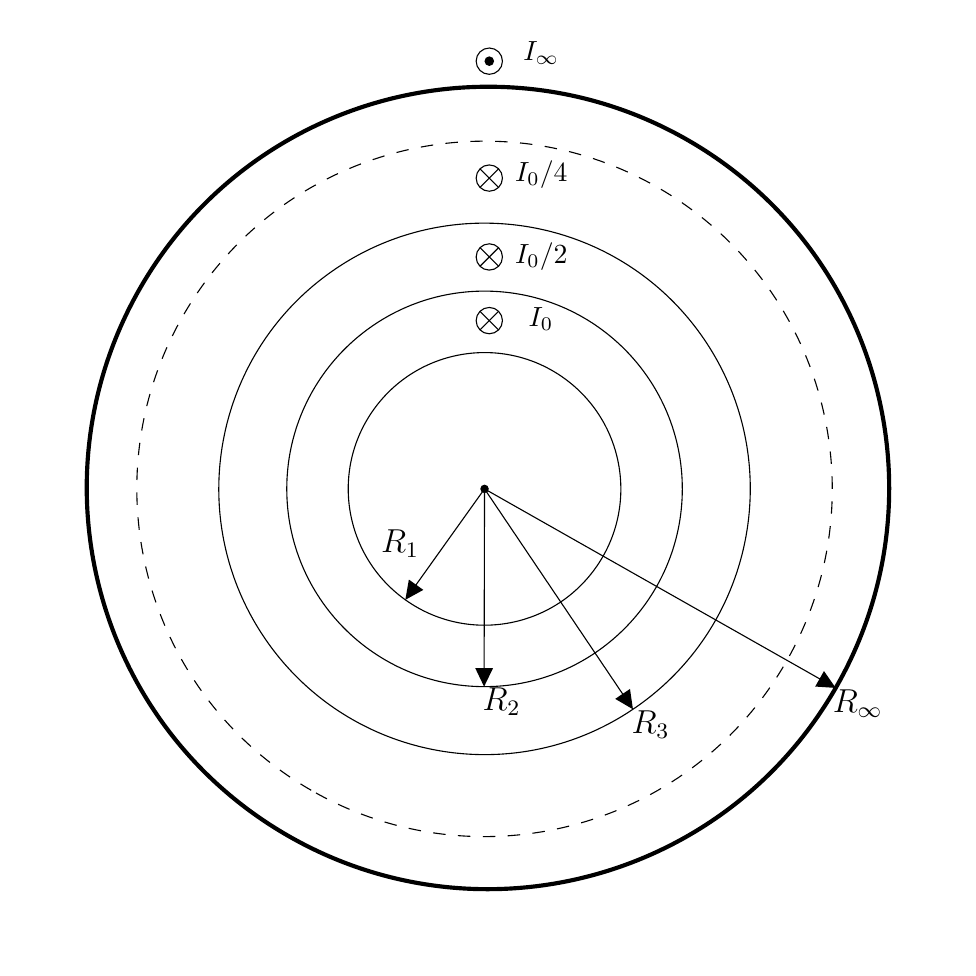
\begin{tikzpicture}[x=0.75pt,y=0.75pt,yscale=-1,xscale=1]
%uncomment if require: \path (0,750); %set diagram left start at 0, and has height of 750

%Shape: Ellipse [id:dp13824326682302956] 
\draw  [line width=1.5]  (242.34,391.51) .. controls (149.81,338.3) and (117.93,220.15) .. (171.14,127.62) .. controls (224.35,35.08) and (342.5,3.2) .. (435.04,56.41) .. controls (527.57,109.62) and (559.45,227.77) .. (506.24,320.31) .. controls (453.03,412.85) and (334.88,444.72) .. (242.34,391.51) -- cycle ;
%Shape: Ellipse [id:dp837502442701394] 
\draw   (230.86,295.92) .. controls (191.36,237.28) and (206.88,157.72) .. (265.53,118.22) .. controls (324.17,78.73) and (403.73,94.25) .. (443.22,152.89) .. controls (482.72,211.54) and (467.2,291.09) .. (408.55,330.59) .. controls (349.91,370.09) and (270.35,354.56) .. (230.86,295.92) -- cycle ;
%Shape: Ellipse [id:dp8448296870986023] 
\draw   (241.76,224.19) .. controls (241.87,171.57) and (284.63,129) .. (337.26,129.12) .. controls (389.88,129.24) and (432.45,172) .. (432.33,224.62) .. controls (432.21,277.25) and (389.45,319.81) .. (336.83,319.69) .. controls (284.2,319.57) and (241.64,276.82) .. (241.76,224.19) -- cycle ;
%Shape: Ellipse [id:dp26024732103447334] 
\draw   (283.6,186.24) .. controls (304.67,156.73) and (345.69,149.89) .. (375.2,170.96) .. controls (404.72,192.04) and (411.56,233.05) .. (390.49,262.57) .. controls (369.41,292.09) and (328.39,298.93) .. (298.88,277.85) .. controls (269.36,256.77) and (262.52,215.76) .. (283.6,186.24) -- cycle ;
%Straight Lines [id:da9435394682627205] 
\draw    (337.04,224.41) -- (503.63,318.83) ;
\draw [shift={(506.24,320.31)}, rotate = 209.54] [fill={rgb, 255:red, 0; green, 0; blue, 0 }  ][line width=0.08]  [draw opacity=0] (8.93,-4.29) -- (0,0) -- (8.93,4.29) -- cycle    ;
%Straight Lines [id:da24753613833187926] 
\draw    (337.04,224.41) -- (406.88,328.1) ;
\draw [shift={(408.55,330.59)}, rotate = 236.04] [fill={rgb, 255:red, 0; green, 0; blue, 0 }  ][line width=0.08]  [draw opacity=0] (8.93,-4.29) -- (0,0) -- (8.93,4.29) -- cycle    ;
%Straight Lines [id:da9326198768496756] 
\draw    (337.04,224.41) -- (336.83,316.69) ;
\draw [shift={(336.83,319.69)}, rotate = 270.13] [fill={rgb, 255:red, 0; green, 0; blue, 0 }  ][line width=0.08]  [draw opacity=0] (8.93,-4.29) -- (0,0) -- (8.93,4.29) -- cycle    ;
%Straight Lines [id:da6485651860835373] 
\draw    (337.04,224.41) -- (300.62,275.41) ;
\draw [shift={(298.88,277.85)}, rotate = 305.53] [fill={rgb, 255:red, 0; green, 0; blue, 0 }  ][line width=0.08]  [draw opacity=0] (8.93,-4.29) -- (0,0) -- (8.93,4.29) -- cycle    ;
%Shape: Ellipse [id:dp17127556547212408] 
\draw  [dash pattern={on 4.5pt off 4.5pt}] (253.54,369.62) .. controls (173.35,323.5) and (145.72,221.11) .. (191.83,140.91) .. controls (237.95,60.71) and (340.34,33.08) .. (420.54,79.2) .. controls (500.74,125.31) and (528.37,227.71) .. (482.25,307.91) .. controls (436.14,388.1) and (333.74,415.73) .. (253.54,369.62) -- cycle ;
%Shape: Ellipse [id:dp12265266084161985] 
\draw   (333,18.33) .. controls (333,14.84) and (335.84,12) .. (339.33,12) .. controls (342.83,12) and (345.67,14.84) .. (345.67,18.33) .. controls (345.67,21.83) and (342.83,24.67) .. (339.33,24.67) .. controls (335.84,24.67) and (333,21.83) .. (333,18.33) -- cycle ;
%Shape: Ellipse [id:dp14680452262194787] 
\draw  [fill={rgb, 255:red, 0; green, 0; blue, 0 }  ,fill opacity=1 ] (337.31,18.33) .. controls (337.31,17.21) and (338.21,16.31) .. (339.33,16.31) .. controls (340.45,16.31) and (341.36,17.21) .. (341.36,18.33) .. controls (341.36,19.45) and (340.45,20.36) .. (339.33,20.36) .. controls (338.21,20.36) and (337.31,19.45) .. (337.31,18.33) -- cycle ;

%Flowchart: Summing Junction [id:dp7499895134813164] 
\draw   (345.67,74.67) .. controls (345.67,71.17) and (342.83,68.33) .. (339.33,68.33) .. controls (335.84,68.33) and (333,71.17) .. (333,74.67) .. controls (333,78.16) and (335.84,81) .. (339.33,81) .. controls (342.83,81) and (345.67,78.16) .. (345.67,74.67) -- cycle ; \draw   (343.81,70.19) -- (334.85,79.15) ; \draw   (334.85,70.19) -- (343.81,79.15) ;
%Flowchart: Summing Junction [id:dp1987512427943714] 
\draw   (345.67,112.67) .. controls (345.67,109.17) and (342.83,106.33) .. (339.33,106.33) .. controls (335.84,106.33) and (333,109.17) .. (333,112.67) .. controls (333,116.16) and (335.84,119) .. (339.33,119) .. controls (342.83,119) and (345.67,116.16) .. (345.67,112.67) -- cycle ; \draw   (343.81,108.19) -- (334.85,117.15) ; \draw   (334.85,108.19) -- (343.81,117.15) ;
%Flowchart: Summing Junction [id:dp06310139127124526] 
\draw   (345.67,143.33) .. controls (345.67,139.84) and (342.83,137) .. (339.33,137) .. controls (335.84,137) and (333,139.84) .. (333,143.33) .. controls (333,146.83) and (335.84,149.67) .. (339.33,149.67) .. controls (342.83,149.67) and (345.67,146.83) .. (345.67,143.33) -- cycle ; \draw   (343.81,138.85) -- (334.85,147.81) ; \draw   (334.85,138.85) -- (343.81,147.81) ;
%Shape: Circle [id:dp8544098462479419] 
\draw  [fill={rgb, 255:red, 0; green, 0; blue, 0 }  ,fill opacity=1 ] (335.29,224.41) .. controls (335.29,225.37) and (336.07,226.16) .. (337.04,226.16) .. controls (338.01,226.16) and (338.79,225.37) .. (338.79,224.41) .. controls (338.79,223.44) and (338.01,222.66) .. (337.04,222.66) .. controls (336.07,222.66) and (335.29,223.44) .. (335.29,224.41) -- cycle ;

% Text Node
\draw (354.54,7.55) node [anchor=north west][inner sep=0.75pt]  [font=\normalsize]  {$I_{\infty}$};
% Text Node
\draw (350.54,104.6) node [anchor=north west][inner sep=0.75pt]  [font=\normalsize]  {$I_{0} /2$};
% Text Node
\draw (350.54,64.91) node [anchor=north west][inner sep=0.75pt]  [font=\normalsize]  {$I_{0} /4$};
% Text Node
\draw (357.04,135.61) node [anchor=north west][inner sep=0.75pt]  [font=\normalsize]  {$I_{0}{}$};
% Text Node
\draw (286.01,243.08) node [anchor=north west][inner sep=0.75pt]  [font=\large]  {$R_{1}$};
% Text Node
\draw (334.89,319.16) node [anchor=north west][inner sep=0.75pt]  [font=\large]  {$R_{2}$};
% Text Node
\draw (406.62,330.05) node [anchor=north west][inner sep=0.75pt]  [font=\large]  {$R_{3}$};
% Text Node
\draw (503.62,319.77) node [anchor=north west][inner sep=0.75pt]  [font=\large]  {$R_{\infty }$};


\end{tikzpicture}

\end{center}


\end{problem}
\begin{flushright}
\textbf{\Large{-Proposed by Nitin Sachan}}
\end{flushright}
\begin{solution}
Magnetic field due to a hollow cylinder will be zero at all interior points and for exterior points hollow cylinder will behave like a wire at the axis. Therefore for the outermost shell at infinity will experience pressure factor of $4$ and due to its own current it will experience a factor of $8$ in pressure expression. Therefore net pressure must be zero in order to make the outermost shell stress free.
$$\frac{\mu_{0} I_{0} I_{\infty}}{4\pi^2 R_{\infty}^2}+\frac{\mu_{0} \left(\frac{I_{0}}{2}\right) I_{\infty}}{4\pi^2 R_{\infty}^2}+\frac{\mu_{0} \left(\frac{I_{0}}{4}\right) I_{\infty}}{4\pi^2 R_{\infty}^2}+\cdots= \frac{\mu_{0} I_{\infty}}{8\pi^2 R_{\infty}^2}$$
$$\mu_{0} I_{0} I_{\infty} \left(1+\frac{1}{2}+\frac{1}{4}+\cdots+\infty\right)=\frac{\mu_{0} I_{\infty}^2}{2}$$
This is a geometric progression with first term 1 and common ratio $1/2$, hence we can write
$$I_{0} \left(\frac{1}{1-\frac{1}{2}}\right)=\frac{I_\infty}{2}$$
$$2I_0 = \frac{I_\infty}{2}$$
$$\boxed{\frac{I_\infty}{I_0}=4}$$
\textbf{Answer : 4}
\end{solution}
\vspace{1cm}%\section{Problem 2}
\begin{problem}

Given a peculiar chain of length 1 m, such that it's
linear density varies as $\lambda(x)=x$, where $x$ is distance from
front edge $A$. It is kept on a table with a small hole
such that the edge A starts falling through it and, the height
of table is $h$. ($g=10 m/s$).

%%%%     Figure      %%%%%%%%%%
 \begin{center}
     

\tikzset{every picture/.style={line width=0.75pt}} %set default line width to 0.75pt        

\begin{tikzpicture}[x=0.75pt,y=0.75pt,yscale=-1,xscale=1]

%Shape: Rectangle [id:dp35625532107225033] 
\draw   (106.82,36.24) -- (498.04,36.24) -- (498.04,47.22) -- (106.82,47.22) -- cycle ;
%Shape: Ellipse [id:dp8513224418902086] 
\draw   (294.81,30.5) .. controls (294.81,28.35) and (297.08,26.61) .. (299.88,26.61) .. controls (302.68,26.61) and (304.95,28.35) .. (304.95,30.5) .. controls (304.95,32.64) and (302.68,34.38) .. (299.88,34.38) .. controls (297.08,34.38) and (294.81,32.64) .. (294.81,30.5) -- cycle ;
%Shape: Ellipse [id:dp6183307303752301] 
\draw   (304.95,30.5) .. controls (304.95,28.35) and (307.22,26.61) .. (310.03,26.61) .. controls (312.83,26.61) and (315.1,28.35) .. (315.1,30.5) .. controls (315.1,32.64) and (312.83,34.38) .. (310.03,34.38) .. controls (307.22,34.38) and (304.95,32.64) .. (304.95,30.5) -- cycle ;
%Shape: Ellipse [id:dp054781232838075455] 
\draw   (300.16,23.38) .. controls (300.16,21.23) and (302.43,19.49) .. (305.24,19.49) .. controls (308.04,19.49) and (310.31,21.23) .. (310.31,23.38) .. controls (310.31,25.52) and (308.04,27.26) .. (305.24,27.26) .. controls (302.43,27.26) and (300.16,25.52) .. (300.16,23.38) -- cycle ;
%Shape: Ellipse [id:dp28287015489818557] 
\draw   (310.03,45.19) .. controls (308.16,45.19) and (306.64,42.58) .. (306.64,39.37) .. controls (306.64,36.15) and (308.16,33.54) .. (310.03,33.54) .. controls (311.89,33.54) and (313.41,36.15) .. (313.41,39.37) .. controls (313.41,42.58) and (311.89,45.19) .. (310.03,45.19) -- cycle ;
%Shape: Ellipse [id:dp44157674508282985] 
\draw   (310.03,56.85) .. controls (308.16,56.85) and (306.64,54.24) .. (306.64,51.02) .. controls (306.64,47.8) and (308.16,45.19) .. (310.03,45.19) .. controls (311.89,45.19) and (313.41,47.8) .. (313.41,51.02) .. controls (313.41,54.24) and (311.89,56.85) .. (310.03,56.85) -- cycle ;
%Shape: Ellipse [id:dp7298072780299072] 
\draw   (310.03,68.5) .. controls (308.16,68.5) and (306.64,65.89) .. (306.64,62.67) .. controls (306.64,59.46) and (308.16,56.85) .. (310.03,56.85) .. controls (311.89,56.85) and (313.41,59.46) .. (313.41,62.67) .. controls (313.41,65.89) and (311.89,68.5) .. (310.03,68.5) -- cycle ;
%Shape: Ellipse [id:dp4746873071782114] 
\draw   (310.03,79.51) .. controls (308.16,79.51) and (306.64,76.9) .. (306.64,73.68) .. controls (306.64,70.46) and (308.16,67.85) .. (310.03,67.85) .. controls (311.89,67.85) and (313.41,70.46) .. (313.41,73.68) .. controls (313.41,76.9) and (311.89,79.51) .. (310.03,79.51) -- cycle ;
%Shape: Ellipse [id:dp5004101112922121] 
\draw   (310.03,91.16) .. controls (308.16,91.16) and (306.64,88.55) .. (306.64,85.34) .. controls (306.64,82.12) and (308.16,79.51) .. (310.03,79.51) .. controls (311.89,79.51) and (313.41,82.12) .. (313.41,85.34) .. controls (313.41,88.55) and (311.89,91.16) .. (310.03,91.16) -- cycle ;
%Shape: Ellipse [id:dp11826978989377923] 
\draw   (315.1,30.5) .. controls (315.1,28.35) and (317.37,26.61) .. (320.17,26.61) .. controls (322.97,26.61) and (325.24,28.35) .. (325.24,30.5) .. controls (325.24,32.64) and (322.97,34.38) .. (320.17,34.38) .. controls (317.37,34.38) and (315.1,32.64) .. (315.1,30.5) -- cycle ;
%Shape: Ellipse [id:dp0032854818474798986] 
\draw   (313.55,28.81) .. controls (311.81,28.04) and (311.22,24.98) .. (312.23,21.98) .. controls (313.23,18.98) and (315.46,17.17) .. (317.21,17.94) .. controls (318.95,18.71) and (319.54,21.77) .. (318.53,24.77) .. controls (317.53,27.78) and (315.3,29.59) .. (313.55,28.81) -- cycle ;
%Shape: Ellipse [id:dp3549508174469138] 
\draw   (310.26,21.41) .. controls (308.51,20.67) and (307.86,17.63) .. (308.82,14.6) .. controls (309.78,11.58) and (311.98,9.72) .. (313.73,10.46) .. controls (315.49,11.19) and (316.13,14.24) .. (315.18,17.26) .. controls (314.22,20.28) and (312.02,22.14) .. (310.26,21.41) -- cycle ;
%Shape: Ellipse [id:dp1488068681524506] 
\draw   (289.9,34.65) .. controls (288.14,33.91) and (287.5,30.87) .. (288.45,27.84) .. controls (289.41,24.82) and (291.61,22.96) .. (293.37,23.69) .. controls (295.12,24.43) and (295.77,27.47) .. (294.81,30.5) .. controls (293.85,33.52) and (291.65,35.38) .. (289.9,34.65) -- cycle ;
%Shape: Ellipse [id:dp8120040535459017] 
\draw   (295.53,26.63) .. controls (293.78,25.9) and (293.01,23.25) .. (293.81,20.72) .. controls (294.61,18.19) and (296.68,16.73) .. (298.44,17.46) .. controls (300.19,18.2) and (300.97,20.85) .. (300.16,23.38) .. controls (299.36,25.91) and (297.29,27.37) .. (295.53,26.63) -- cycle ;
%Straight Lines [id:da8996504617539451] 
\draw    (325.67,47.22) -- (325.67,103.84) ;
\draw [shift={(325.67,103.84)}, rotate = 270] [color={rgb, 255:red, 0; green, 0; blue, 0 }  ][line width=0.75]    (0,5.59) -- (0,-5.59)   ;
\draw [shift={(325.67,47.22)}, rotate = 270] [color={rgb, 255:red, 0; green, 0; blue, 0 }  ][line width=0.75]    (0,5.59) -- (0,-5.59)   ;
%Straight Lines [id:da05420889167129239] 
\draw    (131.32,47.22) -- (130.48,151.58) ;
%Straight Lines [id:da17857238934313124] 
\draw    (469.31,47.22) -- (468.46,151.58) ;
%Straight Lines [id:da12137654389665609] 
\draw    (456.63,47.65) -- (455.79,152) ;
%Straight Lines [id:da7658244327929771] 
\draw    (144,47.22) -- (143.15,151.58) ;
%Straight Lines [id:da12150046416595917] 
\draw    (95.83,47.65) -- (94.99,150.73) ;
\draw [shift={(94.99,150.73)}, rotate = 270.47] [color={rgb, 255:red, 0; green, 0; blue, 0 }  ][line width=0.75]    (0,5.59) -- (0,-5.59)   ;
\draw [shift={(95.83,47.65)}, rotate = 270.47] [color={rgb, 255:red, 0; green, 0; blue, 0 }  ][line width=0.75]    (0,5.59) -- (0,-5.59)   ;
%Shape: Ellipse [id:dp057968954440797305] 
\draw   (310.03,102.82) .. controls (308.16,102.82) and (306.64,100.21) .. (306.64,96.99) .. controls (306.64,93.77) and (308.16,91.16) .. (310.03,91.16) .. controls (311.89,91.16) and (313.41,93.77) .. (313.41,96.99) .. controls (313.41,100.21) and (311.89,102.82) .. (310.03,102.82) -- cycle ;
%Shape: Ellipse [id:dp5238375178734451] 
\draw   (283.82,31.1) .. controls (282.07,30.36) and (281.3,27.72) .. (282.1,25.18) .. controls (282.9,22.65) and (284.97,21.2) .. (286.73,21.93) .. controls (288.48,22.66) and (289.26,25.31) .. (288.45,27.84) .. controls (287.65,30.37) and (285.58,31.83) .. (283.82,31.1) -- cycle ;


% Text Node
\draw (329.8,70.04) node [anchor=north west][inner sep=0.75pt]    {$x$};
% Text Node
\draw (75.47,90.32) node [anchor=north west][inner sep=0.75pt]    {$h$};


\end{tikzpicture}

 \end{center}
%%%%    End Figure      %%%%%%%%%%
 
 \vspace{5mm}
A) When $h>1m>x$, then $v(x)=2 \sqrt{x}$.\\
B) When $h>x>1m$, then $x(t)=5t^2+2t+1$.\\
C) When $1 m>h$, $a(t)=$ is dependent of time.\\
D) When $1 m>h$, $a(t)$ is independent of time.
\end{problem}
\begin{flushright}
\textbf{\Large{-Proposed by Atharva Nilesh Mahajan}}
\end{flushright}
\begin{solution}
When $h>1m>x$:\
We get $$F= mg- v\frac{dm}{dt}$$
$$a= g- \frac{v}{m}\frac{dm}{dt}$$
\begin{equation}
\label{eqn:1}
v \frac{dv}{dx} = g- v\frac{\frac{dm}{dt}}{m}
\end{equation}

Now, using $\lambda(x)=x$, $$dm = x dx$$
Integrating:
$$m = \frac{x^2}{2}$$
Now substituting in (\ref{eqn:1}), we get:

\[v \frac{dv}{dx}=g-\frac{v^2x}{x^2/2}=10-\frac{2v^2}{x}\]

\[\implies v=2\sqrt{x}\]

\vspace{3mm}

When $x=1m$, velocity $= 2 m/s$, and $a=g=10 m/s^2$

\[x-1=vt+\frac{1}{2}at^2\]

\[x-1=2t+5t^2\]

\[x=5t^2+2t+1\]

\[v=10t+2\]

\vspace{3mm}

When the string is not on the ground yet, $a(t)=2 m/s^2$ 

When all of the string falls on the ground, then $a(t)=0 m/s^2$

\textbf{Answers: (A), (B), (C)}

\end{solution}
\vspace{1cm}%\section{Problem 3}
\begin{problem}
\textbf{A Triangular '$L$' story}; 

The self-inductance of an equilateral triangular loop of side $l$ is $L$ (as shown in figure-$I$). A rhombus of one internal angle $60^{\circ}$ and side '$l$' (as shown in figure-$II$) is placed very close to the triangle so that one of their sides align in the same plane (as shown in figure-$III$) \\

A)If the loop in figure-$I$ were of side '$2l$' instead, then its self-inductance would have been '$2L$'. \\

B) The self-inductance of the loop in figure-$II$ is greater than '$2L$'. \\

C) The mutual inductance between the two loops in figure-$III$ is $\frac{L}{3}$\\

D) The mutual inductance between the two loops in figure-$III$ is $\frac{4L}{3}$\\
\begin{center}
    

\tikzset{every picture/.style={line width=0.75pt}} %set default line width to 0.75pt        

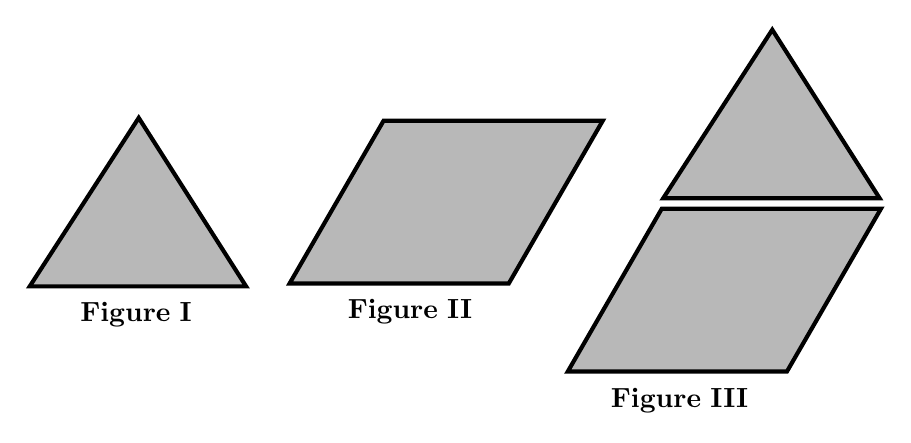
\begin{tikzpicture}[x=0.75pt,y=0.75pt,yscale=-1,xscale=1]
%uncomment if require: \path (0,537); %set diagram left start at 0, and has height of 537

%Shape: Triangle [id:dp4079520034277586] 
\draw  [fill={rgb, 255:red, 0; green, 0; blue, 0 }  ,fill opacity=0.28 ][line width=1.5]  (178.42,51.46) -- (230.14,132.62) -- (125.91,132.62) -- cycle ;
%Shape: Parallelogram [id:dp16119413114025183] 
\draw  [fill={rgb, 255:red, 0; green, 0; blue, 0 }  ,fill opacity=0.28 ][line width=1.5]  (296.37,52.86) -- (401.96,52.86) -- (356.71,131.23) -- (251.11,131.23) -- cycle ;
%Shape: Parallelogram [id:dp9503146048746192] 
\draw  [fill={rgb, 255:red, 0; green, 0; blue, 0 }  ,fill opacity=0.28 ][line width=1.5]  (430.4,95.26) -- (536,95.26) -- (490.74,173.63) -- (385.15,173.63) -- cycle ;
%Shape: Triangle [id:dp3197231943974652] 
\draw  [fill={rgb, 255:red, 0; green, 0; blue, 0 }  ,fill opacity=0.28 ][line width=1.5]  (483.65,9) -- (535.37,90.16) -- (431.13,90.16) -- cycle ;


% Text Node
\draw (149.02,139.08) node [anchor=north west][inner sep=0.75pt]    {$\mathbf{Figure\ I}$};
% Text Node
\draw (277.87,137.62) node [anchor=north west][inner sep=0.75pt]    {$\mathbf{Figure\ II}$};
% Text Node
\draw (404.67,180.6) node [anchor=north west][inner sep=0.75pt]    {$\mathbf{Figure\ III}$};


\end{tikzpicture}

\end{center}



\end{problem}
\begin{flushright}
\textbf{\Large{-Proposed by Janardanudu Thallaparthi}}
\end{flushright}
\begin{solution}


Divide the lower rhombus into two equilateral triangles. Let the mutual inductance of a pair of an equilateral triangle having a side (adjacent ones) be '$M_{\text{adj}}$' and the ones away be '$M_{\text{away}}$'. We need to solve for $M_{\text{adj}}+M_{\text{away}}$. Dimension analysis helps us realise a triangle of twice the side length has '$2L$' inductance. Taking this as a hint to solve the problem further, we build an extra triangle to the above figure to make it a '$2l$' side equilateral triangle (see the equivalence). \\
\begin{center}
    

\tikzset{every picture/.style={line width=0.75pt}} %set default line width to 0.75pt        

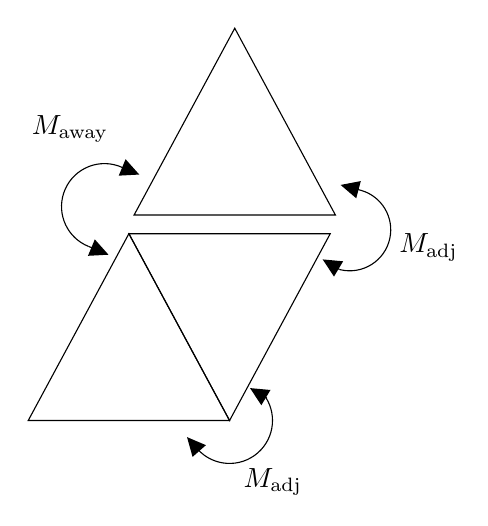
\begin{tikzpicture}[x=0.75pt,y=0.75pt,yscale=-1,xscale=1]
%uncomment if require: \path (0,300); %set diagram left start at 0, and has height of 300

%Shape: Triangle [id:dp45070517116788844] 
\draw   (204,115) -- (252.5,205) -- (155.5,205) -- cycle ;
%Shape: Triangle [id:dp9654711726051111] 
\draw   (252.5,205) -- (204,115) -- (301,115) -- cycle ;
%Shape: Triangle [id:dp9637996023047706] 
\draw   (255,16) -- (303.5,106) -- (206.5,106) -- cycle ;
%Shape: Arc [id:dp9006265533237994] 
\draw  [draw opacity=0] (184.51,121.1) .. controls (174.44,117.06) and (169.14,105.83) .. (172.59,95.4) .. controls (176.19,84.55) and (187.89,78.68) .. (198.74,82.27) .. controls (198.94,82.34) and (199.14,82.41) .. (199.33,82.48) -- (192.23,101.91) -- cycle ; \draw   (184.51,121.1) .. controls (174.44,117.06) and (169.14,105.83) .. (172.59,95.4) .. controls (176.19,84.55) and (187.89,78.68) .. (198.74,82.27) .. controls (198.94,82.34) and (199.14,82.41) .. (199.33,82.48) ;
%Shape: Arc [id:dp2536457345650631] 
\draw  [draw opacity=0] (268.81,192.27) .. controls (275.49,200.81) and (274.45,213.19) .. (266.22,220.48) .. controls (257.67,228.06) and (244.6,227.27) .. (237.02,218.72) .. controls (236.88,218.57) and (236.74,218.41) .. (236.61,218.25) -- (252.5,205) -- cycle ; \draw   (268.81,192.27) .. controls (275.49,200.81) and (274.45,213.19) .. (266.22,220.48) .. controls (257.67,228.06) and (244.6,227.27) .. (237.02,218.72) .. controls (236.88,218.57) and (236.74,218.41) .. (236.61,218.25) ;
%Shape: Arc [id:dp36041828783112884] 
\draw  [draw opacity=0] (315.92,94.13) .. controls (325.86,97.02) and (331.97,107.19) .. (329.67,117.44) .. controls (327.28,128.08) and (316.71,134.78) .. (306.06,132.39) .. controls (305.87,132.34) and (305.67,132.3) .. (305.48,132.25) -- (310.39,113.11) -- cycle ; \draw   (315.92,94.13) .. controls (325.86,97.02) and (331.97,107.19) .. (329.67,117.44) .. controls (327.28,128.08) and (316.71,134.78) .. (306.06,132.39) .. controls (305.87,132.34) and (305.67,132.3) .. (305.48,132.25) ;
%Straight Lines [id:da6217402842023374] 
\draw    (199.33,82.48) -- (206.23,85.35) ;
\draw [shift={(209,86.5)}, rotate = 202.57999999999998] [fill={rgb, 255:red, 0; green, 0; blue, 0 }  ][line width=0.08]  [draw opacity=0] (8.93,-4.29) -- (0,0) -- (8.93,4.29) -- cycle    ;
%Straight Lines [id:da29960175466769323] 
\draw    (184.51,121.1) -- (191.4,123.97) ;
\draw [shift={(194.17,125.12)}, rotate = 202.57999999999998] [fill={rgb, 255:red, 0; green, 0; blue, 0 }  ][line width=0.08]  [draw opacity=0] (8.93,-4.29) -- (0,0) -- (8.93,4.29) -- cycle    ;
%Straight Lines [id:da8778978516616684] 
\draw    (315.92,94.13) -- (308.9,92.27) ;
\draw [shift={(306,91.5)}, rotate = 374.88] [fill={rgb, 255:red, 0; green, 0; blue, 0 }  ][line width=0.08]  [draw opacity=0] (8.93,-4.29) -- (0,0) -- (8.93,4.29) -- cycle    ;
%Straight Lines [id:da13467515008002184] 
\draw    (305.48,132.25) -- (299.93,128.92) ;
\draw [shift={(297.36,127.38)}, rotate = 390.95] [fill={rgb, 255:red, 0; green, 0; blue, 0 }  ][line width=0.08]  [draw opacity=0] (8.93,-4.29) -- (0,0) -- (8.93,4.29) -- cycle    ;
%Straight Lines [id:da28728369632594175] 
\draw    (270.48,194.25) -- (264.93,190.92) ;
\draw [shift={(262.36,189.38)}, rotate = 390.95] [fill={rgb, 255:red, 0; green, 0; blue, 0 }  ][line width=0.08]  [draw opacity=0] (8.93,-4.29) -- (0,0) -- (8.93,4.29) -- cycle    ;
%Straight Lines [id:da011947815826994335] 
\draw    (236.61,218.25) -- (233.98,215.25) ;
\draw [shift={(232,213)}, rotate = 408.7] [fill={rgb, 255:red, 0; green, 0; blue, 0 }  ][line width=0.08]  [draw opacity=0] (8.93,-4.29) -- (0,0) -- (8.93,4.29) -- cycle    ;

% Text Node
\draw (156,56.9) node [anchor=north west][inner sep=0.75pt]    {$M_{\text{away}}$};
% Text Node
\draw (258,226.9) node [anchor=north west][inner sep=0.75pt]    {$M_{\text{adj}}$};
% Text Node
\draw (333,113.9) node [anchor=north west][inner sep=0.75pt]    {$M_{\text{adj}}$};


\end{tikzpicture}

\end{center}
Each small traingle 'Labelled-$1$' haws one self flux term $L_{i}$, one self flux term $L_{i}$, one $M_{\text{adj}} \cdot i$ term, two $M_{\text{away}} \cdot i$ terms. Labelled-$2$ triangle has one $L_{i}$, three  $M_{\text{adj}} \cdot i$ terms. So, counting properly, \\
$$4L_{i}+6M_{\text{adj}} \cdot i+6M_{\text{away}} \cdot i= 2L_i$$
$$\Rightarrow |M_{\text{adj}}+M_{\text{away}}|= \frac{L}{3}$$

\begin{center}


\tikzset{every picture/.style={line width=0.75pt}} %set default line width to 0.75pt        

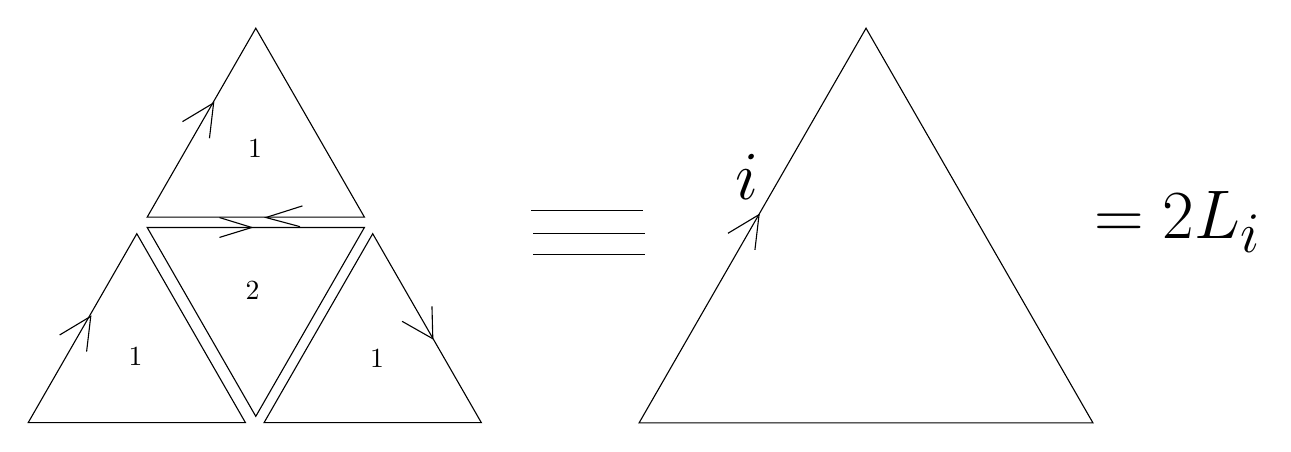
\begin{tikzpicture}[x=0.75pt,y=0.75pt,yscale=-1,xscale=1]
%uncomment if require: \path (0,300); %set diagram left start at 0, and has height of 300

%Shape: Triangle [id:dp40692481476808906] 
\draw   (144.32,20) -- (196.65,111) -- (92,111) -- cycle ;
%Shape: Triangle [id:dp6062532337301327] 
\draw   (144.32,207) -- (92,116) -- (196.65,116) -- cycle ;
%Shape: Triangle [id:dp3087361734769454] 
\draw   (200.65,119) -- (252.97,210) -- (148.32,210) -- cycle ;
%Shape: Triangle [id:dp4678656626426605] 
\draw   (87,119) -- (139.32,210) -- (34.68,210) -- cycle ;
%Straight Lines [id:da6851226797651961] 
\draw    (109,65) -- (124,56) -- (122,73) ;
%Straight Lines [id:da737765955033743] 
\draw    (49.8,167.8) -- (64.8,158.8) -- (62.8,175.8) ;
%Straight Lines [id:da8709391119480012] 
\draw    (126.8,111.2) -- (142.4,116) -- (126.8,120.8) ;
%Straight Lines [id:da1852761866859176] 
\draw    (166.8,105.6) -- (149.2,111.2) -- (165.6,115.6) ;
%Straight Lines [id:da30638262627497226] 
\draw    (229.2,154) -- (229.6,169.6) -- (214.8,161.2) ;

%Straight Lines [id:da8883030152871985] 
\draw    (277,108) -- (331,108) ;
%Straight Lines [id:da7208774874755355] 
\draw    (278,119) -- (332,119) ;
%Straight Lines [id:da6249118764365742] 
\draw    (278,129) -- (332,129) ;

%Shape: Triangle [id:dp03854775186272685] 
\draw   (438.33,20) -- (547.65,210.13) -- (329,210.13) -- cycle ;
%Straight Lines [id:da15276694786846567] 
\draw    (371.8,118.8) -- (386.8,109.8) -- (384.8,126.8) ;


% Text Node
\draw (139.4,72.4) node [anchor=north west][inner sep=0.75pt]    {$1$};
% Text Node
\draw (81.8,172.8) node [anchor=north west][inner sep=0.75pt]    {$1$};
% Text Node
\draw (198.2,173.6) node [anchor=north west][inner sep=0.75pt]    {$1$};
% Text Node
\draw (138.2,140.8) node [anchor=north west][inner sep=0.75pt]    {$2$};
% Text Node
\draw (547,97.4) node [anchor=north west][inner sep=0.75pt]  [font=\Huge]  {$=2L_i$};

% Text Node
\draw (374,79.4) node [anchor=north west][inner sep=0.75pt]  [font=\Huge]  {$i$};


\end{tikzpicture}


\end{center}

\textbf{Answer : (A), (C)}
\end{solution}


\vspace{1cm}%\section{Problem 4}
\begin{problem}

        
\begin{center}


\tikzset{every picture/.style={line width=0.75pt}} %set default line width to 0.75pt        

\begin{tikzpicture}[x=0.75pt,y=0.75pt,yscale=-1,xscale=1]

\draw   (166,61) -- (283,61) -- (283,178) -- (166,178) -- cycle ;
\draw   (140.5,119.5) .. controls (140.5,73.11) and (178.11,35.5) .. (224.5,35.5) .. controls (270.89,35.5) and (308.5,73.11) .. (308.5,119.5) .. controls (308.5,165.89) and (270.89,203.5) .. (224.5,203.5) .. controls (178.11,203.5) and (140.5,165.89) .. (140.5,119.5) -- cycle ;
\draw   (405,64) -- (522,64) -- (522,181) -- (405,181) -- cycle ;
\draw  [fill={rgb, 255:red, 0; green, 0; blue, 0 }  ,fill opacity=1 ] (222.42,119.5) .. controls (222.42,118.35) and (223.35,117.42) .. (224.5,117.42) .. controls (225.65,117.42) and (226.58,118.35) .. (226.58,119.5) .. controls (226.58,120.65) and (225.65,121.58) .. (224.5,121.58) .. controls (223.35,121.58) and (222.42,120.65) .. (222.42,119.5) -- cycle ;
\draw  [fill={rgb, 255:red, 0; green, 0; blue, 0 }  ,fill opacity=1 ] (461.42,122.5) .. controls (461.42,121.35) and (462.35,120.42) .. (463.5,120.42) .. controls (464.65,120.42) and (465.58,121.35) .. (465.58,122.5) .. controls (465.58,123.65) and (464.65,124.58) .. (463.5,124.58) .. controls (462.35,124.58) and (461.42,123.65) .. (461.42,122.5) -- cycle ;

\draw (395,177.73) node [anchor=north west][inner sep=0.75pt]    {$c$};
\draw (473,101.73) node [anchor=north west][inner sep=0.75pt]    {$o$};
\draw (229.67,99.4) node [anchor=north west][inner sep=0.75pt]    {$o$};


\end{tikzpicture}
    
\end{center}

A uniformly charged non-conducting circular disc has its centre at potential $V$. Now a square plate is cut out of this disc keeping its surface charge density same. The new potential at center and corner are $V_o$ and $V_c$ respectively then\par 
A) \quad $V_o=4V_c$\\
B) \quad $V_o=2V_c$\\
C) \quad $V_o=2V \ln (\sqrt{2}+1)$\\
D) \quad $V_o=\frac{2\sqrt{2}}{\pi}V\ln (\sqrt{2}+1)$\\
\end{problem}
\begin{flushright}
\textbf{\Large{-Proposed by Janardanudu Thallaparthi}}
\end{flushright}
\begin{solution}

Dimension analysis leads to $V=KR$. \newline
\begin{center}
    

\tikzset{every picture/.style={line width=0.75pt}} %set default line width to 0.75pt        

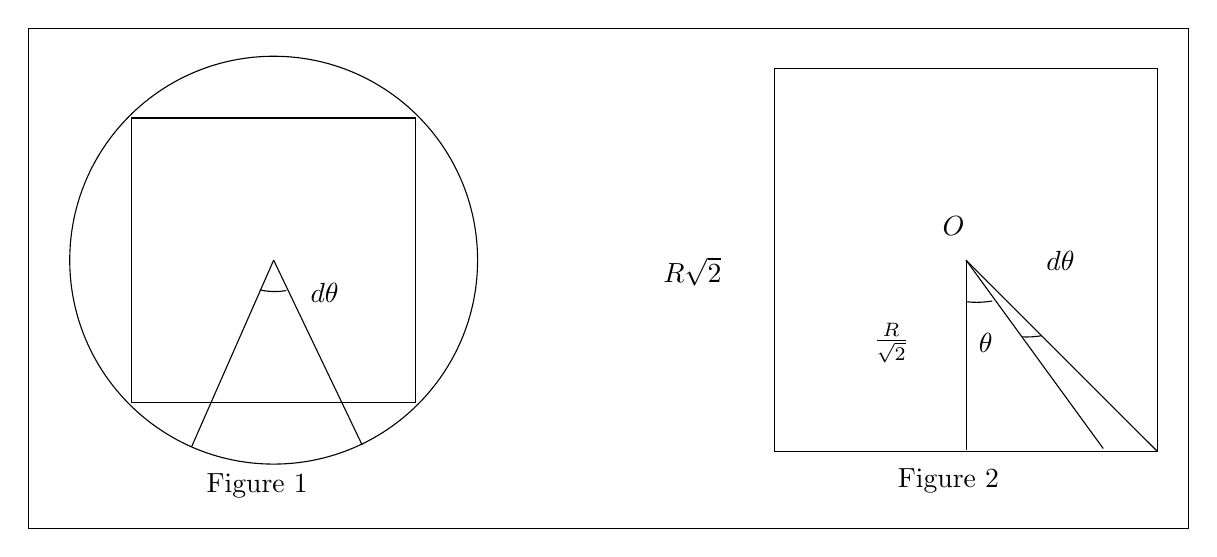
\begin{tikzpicture}[x=0.75pt,y=0.75pt,yscale=-1,xscale=1]
%uncomment if require: \path (0,750); %set diagram left start at 0, and has height of 750

%Shape: Circle [id:dp5413517475921463] 
\draw   (64,151.75) .. controls (64,97.49) and (107.99,53.5) .. (162.25,53.5) .. controls (216.51,53.5) and (260.5,97.49) .. (260.5,151.75) .. controls (260.5,206.01) and (216.51,250) .. (162.25,250) .. controls (107.99,250) and (64,206.01) .. (64,151.75) -- cycle ;
%Shape: Square [id:dp18547171031156617] 
\draw   (93.76,83.26) -- (230.74,83.26) -- (230.74,220.24) -- (93.76,220.24) -- cycle ;
%Straight Lines [id:da9431528644528673] 
\draw    (162.25,151.75) -- (204.9,240.82) ;
%Straight Lines [id:da686029159672902] 
\draw    (162.25,151.75) -- (122.84,241.36) ;
%Shape: Arc [id:dp8797669402858073] 
\draw  [draw opacity=0] (168.39,166.38) .. controls (166.57,166.7) and (164.7,166.87) .. (162.79,166.87) .. controls (160.32,166.87) and (157.92,166.59) .. (155.61,166.07) -- (162.79,134.48) -- cycle ; \draw   (168.39,166.38) .. controls (166.57,166.7) and (164.7,166.87) .. (162.79,166.87) .. controls (160.32,166.87) and (157.92,166.59) .. (155.61,166.07) ;
%Shape: Square [id:dp8693443945428578] 
\draw   (403.69,59.56) -- (588,59.56) -- (588,243.87) -- (403.69,243.87) -- cycle ;
%Straight Lines [id:da9145704907206791] 
\draw    (495.84,151.72) -- (561.94,242.51) ;
%Straight Lines [id:da2007446325297506] 
\draw    (495.84,151.72) -- (495.84,243.24) ;
%Shape: Arc [id:dp7425569777207155] 
\draw  [draw opacity=0] (508.46,171.41) .. controls (506.01,171.83) and (503.5,172.06) .. (500.93,172.06) .. controls (499.38,172.06) and (497.84,171.97) .. (496.34,171.82) -- (500.93,128.47) -- cycle ; \draw   (508.46,171.41) .. controls (506.01,171.83) and (503.5,172.06) .. (500.93,172.06) .. controls (499.38,172.06) and (497.84,171.97) .. (496.34,171.82) ;
%Straight Lines [id:da07967796187084453] 
\draw    (495.84,151.72) -- (588,243.87) ;
%Shape: Arc [id:dp7834750356472047] 
\draw  [draw opacity=0] (532.43,188.11) .. controls (529.98,188.54) and (527.47,188.76) .. (524.9,188.76) .. controls (524.16,188.76) and (523.42,188.74) .. (522.69,188.71) -- (524.9,145.18) -- cycle ; \draw   (532.43,188.11) .. controls (529.98,188.54) and (527.47,188.76) .. (524.9,188.76) .. controls (524.16,188.76) and (523.42,188.74) .. (522.69,188.71) ;
%Shape: Rectangle [id:dp39203512647604066] 
\draw   (44,40) -- (603,40) -- (603,281) -- (44,281) -- cycle ;

% Text Node
\draw (178.74,161.42) node [anchor=north west][inner sep=0.75pt]    {$d\theta $};
% Text Node
\draw (533.28,146.3) node [anchor=north west][inner sep=0.75pt]    {$d\theta $};
% Text Node
\draw (500.74,185.52) node [anchor=north west][inner sep=0.75pt]    {$\theta $};
% Text Node
\draw (483.26,129.59) node [anchor=north west][inner sep=0.75pt]    {$O$};
% Text Node
\draw (449.84,180.92) node [anchor=north west][inner sep=0.75pt]    {$\frac{R}{\sqrt{2}}$};
% Text Node
\draw (348.69,149.11) node [anchor=north west][inner sep=0.75pt]    {$R\sqrt{2}$};
% Text Node
\draw (128.69,253.11) node [anchor=north west][inner sep=0.75pt]    {$\text{Figure 1}$};
% Text Node
\draw (461.69,251.11) node [anchor=north west][inner sep=0.75pt]    {$\text{Figure 2}$};


\end{tikzpicture}

\end{center}






Each $d\theta$ sectors contributes equally. So, $dV=\frac{d\theta}{2\pi} KR$. We use this result in Figure-$2$ for sectors of variable radii given by $\frac{R}{\sqrt{2}}\sec{\theta}$, assuming square to be made of "4" right isosceles plates. So, 
\[V_o = 4 \int_{\frac{-\pi}{4}}^{\frac{\pi}{4}} \frac{d\theta}{2\pi} K\left(\frac{R}{\sqrt{2}}\sec{\theta}\right)\]
\[\implies V_0 = \frac{2\sqrt{2}}{\pi}KR\int_0^{\frac{\pi}{4}}\sec{\theta} d\theta\]
\[\implies V_0 = \frac{2\sqrt{2}}{\pi}KR\ln{\left(\sqrt{2}+1\right)}\]
But $V=KR$, so we can write: \[\boxed{\implies V_0 = \frac{2\sqrt{2}}{\pi}V\ln{\left(\sqrt{2}+1\right)}}\]
\textbf{Answer: (D)}

\end{solution}


\vspace{1cm}%\section{Problem 5}
\begin{problem}

Consider a bead of mass $m=1 kg$ which is rigidly attached to $2$ massless rods at right angles as shown. The lengths of the rods are $2.5 \ m$ and $1\ m$ as shown. Let's say this arrangement is placed on a rough table with $2$ rigid vertical barriers of $v=5\ m s^{-1}$ perpendicular to the barrier, and it finally comes to rest at the position coordinate $(a,b)$ assuming the initial position to be Origin.\\ Find the value of
$$4\cdot|b\sqrt{3}-a|$$ 
If 
$\mu_{\text{table \ and \ bead}} = 0.5, \text{and} g=10 \ m s^{-2}$
\begin{center}
    

\tikzset{every picture/.style={line width=0.75pt}} %set default line width to 0.75pt        
\boxed{
\begin{tikzpicture}[x=0.75pt,y=0.75pt,yscale=-1,xscale=1]
%uncomment if require: \path (0,356); %set diagram left start at 0, and has height of 356

%Shape: Right Angle [id:dp2423931160285837] 
\draw   (163.31,128.73) -- (163.31,54.35) -- (335.2,54.35) ;
%Shape: Right Angle [id:dp6848218796619385] 
\draw   (163.31,68.4) -- (177.35,68.4) -- (177.35,54.35) ;
%Straight Lines [id:da6965341731217758] 
\draw    (163.31,43.61) -- (335.2,43.61) ;
\draw [shift={(335.2,43.61)}, rotate = 540] [color={rgb, 255:red, 0; green, 0; blue, 0 }  ][line width=0.75]    (0,5.59) -- (0,-5.59)   ;
\draw [shift={(163.31,43.61)}, rotate = 540] [color={rgb, 255:red, 0; green, 0; blue, 0 }  ][line width=0.75]    (0,5.59) -- (0,-5.59)   ;
%Straight Lines [id:da4374043284803446] 
\draw    (150.91,54.35) -- (150.91,128.73) ;
\draw [shift={(150.91,128.73)}, rotate = 270] [color={rgb, 255:red, 0; green, 0; blue, 0 }  ][line width=0.75]    (0,5.59) -- (0,-5.59)   ;
\draw [shift={(150.91,54.35)}, rotate = 270] [color={rgb, 255:red, 0; green, 0; blue, 0 }  ][line width=0.75]    (0,5.59) -- (0,-5.59)   ;
%Straight Lines [id:da40715297571097864] 
\draw    (132.2,188.6) -- (305.2,188.6) ;
%Straight Lines [id:da5701959832709445] 
\draw    (132.2,196.6) -- (288.2,196.6) -- (306.2,196.6) ;
%Straight Lines [id:da06361817267733239] 
\draw    (308.2,186.25) -- (308.2,156.6) ;
\draw [shift={(308.2,153.6)}, rotate = 450] [fill={rgb, 255:red, 0; green, 0; blue, 0 }  ][line width=0.08]  [draw opacity=0] (8.93,-4.29) -- (0,0) -- (8.93,4.29) -- cycle    ;
\draw [shift={(308.2,188.6)}, rotate = 270] [color={rgb, 255:red, 0; green, 0; blue, 0 }  ][line width=0.75]      (0, 0) circle [x radius= 3.35, y radius= 3.35]   ;
%Straight Lines [id:da5724253744031245] 
\draw    (385.53,197.6) -- (385.53,188.6) -- (561.53,187.6) ;
%Straight Lines [id:da9900429843401801] 
\draw    (385.2,197.6) -- (561.53,197.6) ;
%Straight Lines [id:da823718755109442] 
\draw    (297.2,248.47) -- (307.2,192.6) ;
%Straight Lines [id:da2926700586689652] 
\draw    (423,203.4) -- (311.2,188.4) ;

% Text Node
\draw (233.73,25.26) node [anchor=north west][inner sep=0.75pt]    {$2.5m$};
% Text Node
\draw (114.94,84.77) node [anchor=north west][inner sep=0.75pt]    {$1m$};
% Text Node
\draw (306.73,135) node [anchor=north west][inner sep=0.75pt]    {$5m/s$};
% Text Node
\draw (309.4,270.33) node [anchor=north west][inner sep=0.75pt]    {$Top\ View$};


\end{tikzpicture}}

\end{center}
\end{problem}
\begin{flushright}
\textbf{\Large{-Proposed by Atharva Shivaram Mahajan}}
\end{flushright}
\begin{solution}
%% Figure 1
\begin{center}
    \tikzset{every picture/.style={line width=0.75pt}} %set default line width to 0.75pt        
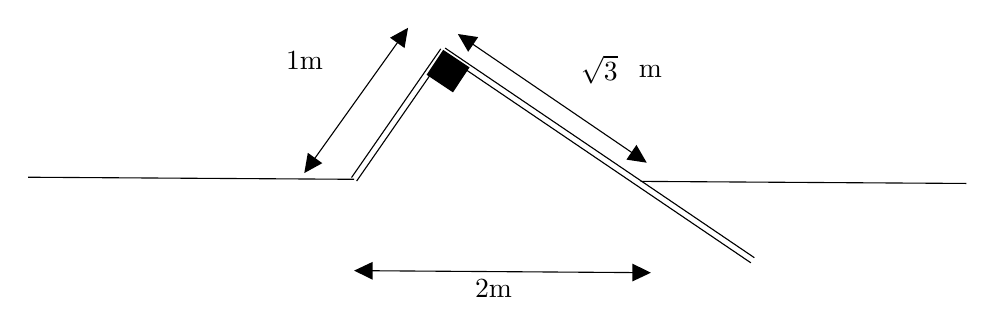
\begin{tikzpicture}[x=0.75pt,y=0.75pt,yscale=-1,xscale=1]
%uncomment if require: \path (0,300); %set diagram left start at 0, and has height of 300
%Straight Lines [id:da711233867243741] 
\draw    (100,118) -- (257,119) ;
%Straight Lines [id:da8574720198051322] 
\draw    (395,120) -- (508.99,120.73) -- (552,121) ;
%Straight Lines [id:da22926251509039042] 
\draw    (255.77,118.15) -- (298.77,56.15)(258.23,119.85) -- (301.23,57.85) ;
%Straight Lines [id:da448616977028955] 
\draw [fill={rgb, 255:red, 0; green, 0; blue, 0 }  ,fill opacity=1 ]   (448.16,159.24) -- (299.16,58.24)(449.84,156.76) -- (300.84,55.76) ;
%Shape: Rectangle [id:dp9153179604750035] 
\draw  [fill={rgb, 255:red, 0; green, 0; blue, 0 }  ,fill opacity=1 ] (300,57) -- (312.25,65.15) -- (304.56,76.73) -- (292.3,68.58) -- cycle ;
%Straight Lines [id:da8887552080956109] 
\draw    (260,163.02) -- (397,163.98) ;
\draw [shift={(400,164)}, rotate = 180.4] [fill={rgb, 255:red, 0; green, 0; blue, 0 }  ][line width=0.08]  [draw opacity=0] (8.93,-4.29) -- (0,0) -- (8.93,4.29) -- cycle    ;
\draw [shift={(257,163)}, rotate = 0.4] [fill={rgb, 255:red, 0; green, 0; blue, 0 }  ][line width=0.08]  [draw opacity=0] (8.93,-4.29) -- (0,0) -- (8.93,4.29) -- cycle    ;
%Straight Lines [id:da97162948128714] 
\draw    (234.74,113.56) -- (281.26,48.44) ;
\draw [shift={(283,46)}, rotate = 485.54] [fill={rgb, 255:red, 0; green, 0; blue, 0 }  ][line width=0.08]  [draw opacity=0] (8.93,-4.29) -- (0,0) -- (8.93,4.29) -- cycle    ;
\draw [shift={(233,116)}, rotate = 305.54] [fill={rgb, 255:red, 0; green, 0; blue, 0 }  ][line width=0.08]  [draw opacity=0] (8.93,-4.29) -- (0,0) -- (8.93,4.29) -- cycle    ;
%Straight Lines [id:da2997316618055039] 
\draw    (395.52,109.31) -- (309.48,50.69) ;
\draw [shift={(307,49)}, rotate = 394.27] [fill={rgb, 255:red, 0; green, 0; blue, 0 }  ][line width=0.08]  [draw opacity=0] (8.93,-4.29) -- (0,0) -- (8.93,4.29) -- cycle    ;
\draw [shift={(398,111)}, rotate = 214.27] [fill={rgb, 255:red, 0; green, 0; blue, 0 }  ][line width=0.08]  [draw opacity=0] (8.93,-4.29) -- (0,0) -- (8.93,4.29) -- cycle    ;
% Text Node
\draw (314,166) node [anchor=north west][inner sep=0.75pt]   [align=left] {2m};
% Text Node
\draw (223,56) node [anchor=north west][inner sep=0.75pt]   [align=left] {1m\\};
% Text Node
\draw (365,58) node [anchor=north west][inner sep=0.75pt]    {$\sqrt{3}$};
% Text Node
\draw (393,63) node [anchor=north west][inner sep=0.75pt]   [align=left] {m};
\end{tikzpicture}
\end{center}
First of all, observe that the locus of the particle will be circular initially.

In this time, its speed will decrease at a constant rate of $\mu g \hspace{2mm} m/s^2$

\vspace{2mm}

After this point, it will go in a straight line as the length of one rod is just $1 m$

\begin{equation}
    \begin{split}
        v^2 & = u^2-2as_1 \\
            & = 5^2-2 \cdot (0.5 \cdot10)\cdot \frac{\pi r}{3} 
    \end{split}
\end{equation}

\begin{equation}
    \boxed{v=\sqrt{25-10 \cdot \frac{\pi}{3}}}
\end{equation}

After this, distance travelled will be

\[0=v^2-2as_2\]

\[\implies s_2=\sqrt{\frac{v^2}{2a}}=\sqrt{\frac{{25-10 \cdot \frac{\pi}{3}}}{2 \cdot (0.5 \cdot10)}}=\sqrt{\frac{25-10\frac{\pi}{3}}{10}}\]

\begin{equation}
    \boxed{s_2=\sqrt{\frac{5}{2}-\frac{\pi}{3}}}
\end{equation}

Final coordinate will be:

\[(\cos(60)+s_2 \cos(30) , \hspace{1mm} \sin(60)+s_2 \sin(30))\]
\[=\Bigg(\frac{1}{2}+\sqrt{\frac{5}{2}-\frac{\pi}{3}} \cdot \frac{\sqrt{3}}{2}, \hspace{1mm} \frac{\sqrt{3}}{2}+\sqrt{\frac{5}{2}- \frac{\pi}{3}} \cdot \frac{1}{2}\Bigg)\]

So, 

\[4 |b \sqrt{3}-a|=4 \Bigg|\frac{3}{2}+\sqrt{\frac{5}{2}- \frac{\pi}{3}} \cdot \frac{\sqrt{3}}{2}-\frac{1}{2}-\sqrt{\frac{5}{2}- \frac{\pi}{3}} \cdot \frac{\sqrt{3}}{2}\Bigg|\]


\boxed{\text{Ans}: 4}
%% Figure 2
\begin{center}
    

\tikzset{every picture/.style={line width=0.75pt}} %set default line width to 0.75pt        

\begin{tikzpicture}[x=0.75pt,y=0.75pt,yscale=-1,xscale=1]
%uncomment if require: \path (0,300); %set diagram left start at 0, and has height of 300

%Straight Lines [id:da711233867243741] 
\draw    (2,143.17) -- (230.71,144.63) ;
%Straight Lines [id:da8574720198051322] 
\draw    (431.74,146.08) -- (597.79,147.14) -- (660.45,147.54) ;
%Straight Lines [id:da22926251509039042] 
\draw [color={rgb, 255:red, 140; green, 14; blue, 252 }  ,draw opacity=1 ][fill={rgb, 255:red, 255; green, 0; blue, 0 }  ,fill opacity=1 ]   (229.48,143.77) -- (292.12,53.45)(231.94,145.48) -- (294.58,55.16) ;
%Shape: Arc [id:dp09390960457131636] 
\draw  [draw opacity=0] (231.35,146.08) .. controls (231.35,145.73) and (231.35,145.39) .. (231.35,145.04) .. controls (231.93,89.88) and (277.11,45.63) .. (332.27,46.21) .. controls (387.43,46.79) and (431.67,91.97) .. (431.1,147.13) .. controls (431.09,147.73) and (431.08,148.34) .. (431.06,148.94) -- (331.22,146.08) -- cycle ; \draw   (231.35,146.08) .. controls (231.35,145.73) and (231.35,145.39) .. (231.35,145.04) .. controls (231.93,89.88) and (277.11,45.63) .. (332.27,46.21) .. controls (387.43,46.79) and (431.67,91.97) .. (431.1,147.13) .. controls (431.09,147.73) and (431.08,148.34) .. (431.06,148.94) ;
%Straight Lines [id:da019158372781863164] 
\draw [color={rgb, 255:red, 255; green, 8; blue, 8 }  ,draw opacity=1 ]   (230.71,144.63) -- (230.71,79.62) ;
\draw [shift={(230.71,77.62)}, rotate = 450] [color={rgb, 255:red, 255; green, 8; blue, 8 }  ,draw opacity=1 ][line width=0.75]    (10.93,-3.29) .. controls (6.95,-1.4) and (3.31,-0.3) .. (0,0) .. controls (3.31,0.3) and (6.95,1.4) .. (10.93,3.29)   ;
%Straight Lines [id:da6400107435780602] 
\draw [color={rgb, 255:red, 246; green, 0; blue, 0 }  ,draw opacity=1 ]   (293.35,54.31) -- (346.86,31.78) ;
\draw [shift={(348.71,31)}, rotate = 517.1700000000001] [color={rgb, 255:red, 246; green, 0; blue, 0 }  ,draw opacity=1 ][line width=0.75]    (10.93,-3.29) .. controls (6.95,-1.4) and (3.31,-0.3) .. (0,0) .. controls (3.31,0.3) and (6.95,1.4) .. (10.93,3.29)   ;
%Straight Lines [id:da6946145063260911] 
\draw  [dash pattern={on 0.84pt off 2.51pt}]  (230.71,144.63) -- (431.74,146.08) ;
%Shape: Circle [id:dp8427051743011251] 
\draw  [fill={rgb, 255:red, 0; green, 0; blue, 0 }  ,fill opacity=1 ] (329.22,145.35) .. controls (329.22,144.25) and (330.12,143.35) .. (331.22,143.35) .. controls (332.33,143.35) and (333.22,144.25) .. (333.22,145.35) .. controls (333.22,146.46) and (332.33,147.35) .. (331.22,147.35) .. controls (330.12,147.35) and (329.22,146.46) .. (329.22,145.35) -- cycle ;
%Straight Lines [id:da27290473589018815] 
\draw  [dash pattern={on 4.5pt off 4.5pt}]  (293.35,54.31) -- (331.22,145.35) ;
%Straight Lines [id:da0371987429410201] 
\draw  [dash pattern={on 4.5pt off 4.5pt}]  (230.71,144.63) -- (329.22,145.35) ;
%Shape: Arc [id:dp6875478093811267] 
\draw  [draw opacity=0] (309.93,145.01) .. controls (309.83,144.38) and (309.78,143.73) .. (309.78,143.07) .. controls (309.78,137.03) and (314.08,132.14) .. (319.39,132.14) .. controls (321.29,132.14) and (323.06,132.76) .. (324.55,133.84) -- (319.39,143.07) -- cycle ; \draw   (309.93,145.01) .. controls (309.83,144.38) and (309.78,143.73) .. (309.78,143.07) .. controls (309.78,137.03) and (314.08,132.14) .. (319.39,132.14) .. controls (321.29,132.14) and (323.06,132.76) .. (324.55,133.84) ;
%Straight Lines [id:da22017865510269963] 
\draw    (236,159.06) -- (330,160.94) ;
\draw [shift={(333,161)}, rotate = 181.15] [fill={rgb, 255:red, 0; green, 0; blue, 0 }  ][line width=0.08]  [draw opacity=0] (8.93,-4.29) -- (0,0) -- (8.93,4.29) -- cycle    ;
\draw [shift={(233,159)}, rotate = 1.15] [fill={rgb, 255:red, 0; green, 0; blue, 0 }  ][line width=0.08]  [draw opacity=0] (8.93,-4.29) -- (0,0) -- (8.93,4.29) -- cycle    ;
%Straight Lines [id:da5564189152636927] 
\draw  [dash pattern={on 0.84pt off 2.51pt}]  (293.35,54.31) -- (404,56) ;
%Shape: Free Drawing [id:dp703247676082269] 
\draw  [color={rgb, 255:red, 0; green, 0; blue, 0 }  ][line width=0.75] [line join = round][line cap = round] (318,48) .. controls (318,51.33) and (318,61.33) .. (318,58) .. controls (318,54.33) and (318.56,50.62) .. (318,47) .. controls (317.78,45.6) and (314.37,42.74) .. (315,44) .. controls (316.97,47.94) and (319,48.69) .. (319,54) ;
%Shape: Free Drawing [id:dp2465244774746833] 
\draw  [color={rgb, 255:red, 0; green, 0; blue, 0 }  ][line width=0.75] [line join = round][line cap = round] (314,45) .. controls (319.59,45) and (317,56.13) .. (317,56) .. controls (317,52.65) and (317.5,49) .. (316,46) .. controls (315.94,45.87) and (315.24,41.76) .. (314,43) .. controls (313.59,43.41) and (316,47.37) .. (316,48) ;

% Text Node
\draw (287,117) node [anchor=north west][inner sep=0.75pt]    {$60^{\circ }$};
% Text Node
\draw (270,159) node [anchor=north west][inner sep=0.75pt]    {$1m$};
% Text Node
\draw (262.03,99.47) node [anchor=north west][inner sep=0.75pt]    {$1m$};
% Text Node
\draw (208,94) node [anchor=north west][inner sep=0.75pt]  [font=\Large]  {$v$};
% Text Node
\draw (306,11) node [anchor=north west][inner sep=0.75pt]  [font=\Large]  {$v$};
% Text Node
\draw (321.03,42.65) node [anchor=north west][inner sep=0.75pt]  [font=\small]  {$30^{\circ }$};


\end{tikzpicture}
\end{center}
\end{solution}
\vspace{1cm}%\section{Problem 6}
\begin{problem}

Consider a very low-resistivity fluid. The magnetic field is at time $t=0$ sec is given by : $\vec{B}$
=$B_0$ $\vec{e_y}$. The velocity field is $\vec{V}= \frac{1}{1+\left(\frac{y}{m}\right)^2} \ \vec{e_x}\  m/s$ always.\\\
What is the magnitude of magnetic field at $(0,1)m$ at $t=1$ second?

$A) B_0 $\\
$B) B_0 /2$\\
$C) \sqrt{3} B_0/2$\\
$D) \sqrt{5} B_0/2$


\end{problem}
\begin{flushright}
\textbf{\Large{-Proposed by Hemansh Shah}}
\end{flushright}
\begin{solution}
For a low resistivity fluid, consider a bunch of fluid elements forming a loop. As the fluid moves, the loop changes shape, expands/contacts, etc.\par
If the magnetic field through the loop changes, there is an electric field curl induced. But, that leads to the flow of current, which opposes the change in magnetic field. In the limit of very low resistivity, the magnetic field through the loop can not change. It stays a constant.\par
Now, let us consider two loops at $t=0$ in the fluid as shown.\par
\begin{center}
\tikzset{every picture/.style={line width=0.75pt}} %set default line width to 0.75pt

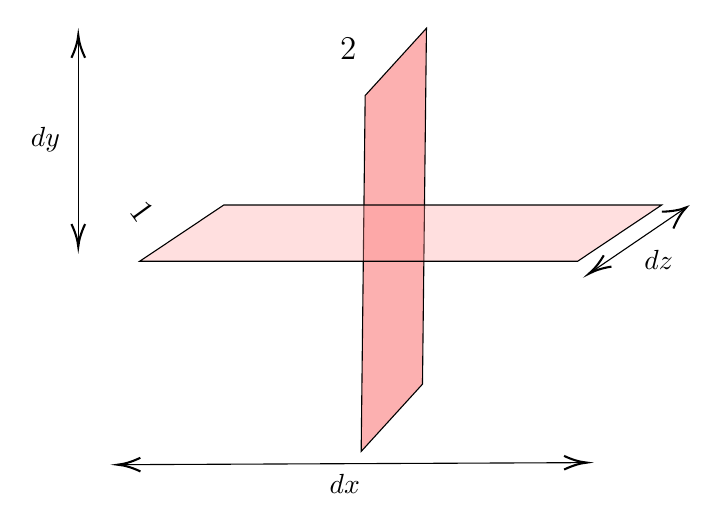
\begin{tikzpicture}[x=0.75pt,y=0.75pt,yscale=-1,xscale=1]
%uncomment if require: \path (0,300); %set diagram left start at 0, and has height of 300

%Flowchart: Data [id:dp7035880816369227] 
\draw  [fill={rgb, 255:red, 246; green, 0; blue, 0 }  ,fill opacity=0.31 ] (219.34,41.25) -- (248.87,8.82) -- (246.95,180.3) -- (217.41,212.73) -- cycle ;
%Shape: Rectangle [id:dp04887569784950463] 
\draw  [fill={rgb, 255:red, 255; green, 149; blue, 149 }  ,fill opacity=0.3 ] (151.2,94) -- (362.19,94) -- (321.68,121.11) -- (110.69,121.11) -- cycle ;
%Straight Lines [id:da09905766820455364] 
\draw    (372.45,96.23) -- (328.76,125.98) ;
\draw [shift={(327.11,127.11)}, rotate = 325.75] [color={rgb, 255:red, 0; green, 0; blue, 0 }  ][line width=0.75]    (10.93,-3.29) .. controls (6.95,-1.4) and (3.31,-0.3) .. (0,0) .. controls (3.31,0.3) and (6.95,1.4) .. (10.93,3.29)   ;
\draw [shift={(374.11,95.11)}, rotate = 145.75] [color={rgb, 255:red, 0; green, 0; blue, 0 }  ][line width=0.75]    (10.93,-4.9) .. controls (6.95,-2.3) and (3.31,-0.67) .. (0,0) .. controls (3.31,0.67) and (6.95,2.3) .. (10.93,4.9)   ;
%Straight Lines [id:da7533540101666225] 
\draw    (81.11,112.11) -- (81.11,14.11) ;
\draw [shift={(81.11,12.11)}, rotate = 450] [color={rgb, 255:red, 0; green, 0; blue, 0 }  ][line width=0.75]    (10.93,-3.29) .. controls (6.95,-1.4) and (3.31,-0.3) .. (0,0) .. controls (3.31,0.3) and (6.95,1.4) .. (10.93,3.29)   ;
\draw [shift={(81.11,114.11)}, rotate = 270] [color={rgb, 255:red, 0; green, 0; blue, 0 }  ][line width=0.75]    (10.93,-3.29) .. controls (6.95,-1.4) and (3.31,-0.3) .. (0,0) .. controls (3.31,0.3) and (6.95,1.4) .. (10.93,3.29)   ;
%Straight Lines [id:da901491630243338] 
\draw    (102.11,219.1) -- (324.11,218.12) ;
\draw [shift={(326.11,218.11)}, rotate = 539.75] [color={rgb, 255:red, 0; green, 0; blue, 0 }  ][line width=0.75]    (10.93,-3.29) .. controls (6.95,-1.4) and (3.31,-0.3) .. (0,0) .. controls (3.31,0.3) and (6.95,1.4) .. (10.93,3.29)   ;
\draw [shift={(100.11,219.11)}, rotate = 359.75] [color={rgb, 255:red, 0; green, 0; blue, 0 }  ][line width=0.75]    (10.93,-3.29) .. controls (6.95,-1.4) and (3.31,-0.3) .. (0,0) .. controls (3.31,0.3) and (6.95,1.4) .. (10.93,3.29)   ;

% Text Node
\draw (113.8,89.28) node [anchor=north west][inner sep=0.75pt]  [font=\large,rotate=-53.78]  {$1$};
% Text Node
\draw (201,222.4) node [anchor=north west][inner sep=0.75pt]    {$dx$};
% Text Node
\draw (57,55.4) node [anchor=north west][inner sep=0.75pt]    {$dy$};
% Text Node
\draw (352.61,114.51) node [anchor=north west][inner sep=0.75pt]    {$dz$};
% Text Node
\draw (206,12.4) node [anchor=north west][inner sep=0.75pt]  [font=\large]  {$2$};

\end{tikzpicture}  
\end{center}
The loop $1$ has flux $B_0 dx dz$ through it, Whereas loop $2$ has flux $0$ through it.\par
Now, let us look at where these loops will end up after a time $t$ and how they will look.\par
The loops are moved ahead by $vt$, and oriented as shown below: \par
\begin{center}
\tikzset{every picture/.style={line width=0.75pt}} %set default line width to 0.75pt

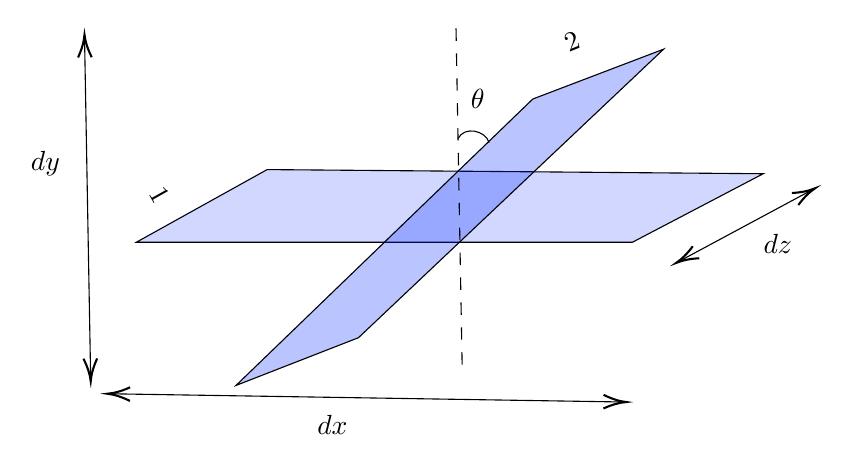
\begin{tikzpicture}[x=0.75pt,y=0.75pt,yscale=-1,xscale=1]
%uncomment if require: \path (0,300); %set diagram left start at 0, and has height of 300

%Shape: Polygon [id:ds916886588727925] 
\draw  [fill={rgb, 255:red, 0; green, 31; blue, 255 }  ,fill opacity=0.18 ] (204.11,116.47) -- (443.11,118.47) -- (380.11,151.47) -- (141.11,151.47) -- cycle ;
%Shape: Polygon [id:ds05642300854837812] 
\draw  [fill={rgb, 255:red, 0; green, 40; blue, 255 }  ,fill opacity=0.27 ] (395.11,58.47) -- (332.11,82.47) -- (189.11,220.47) -- (248.11,197.47) -- cycle ;
%Straight Lines [id:da3195531099085156] 
\draw  [dash pattern={on 4.5pt off 4.5pt}]  (295.11,48.47) -- (298.11,213.47) ;
%Curve Lines [id:da3017736924368517] 
\draw    (311.11,103.47) .. controls (309.11,97.47) and (299.11,95.47) .. (296.11,101.47) ;
%Straight Lines [id:da5840092338247029] 
\draw    (402.87,160.52) -- (466.35,126.42) ;
\draw [shift={(468.11,125.47)}, rotate = 511.75] [color={rgb, 255:red, 0; green, 0; blue, 0 }  ][line width=0.75]    (10.93,-3.29) .. controls (6.95,-1.4) and (3.31,-0.3) .. (0,0) .. controls (3.31,0.3) and (6.95,1.4) .. (10.93,3.29)   ;
\draw [shift={(401.11,161.47)}, rotate = 331.75] [color={rgb, 255:red, 0; green, 0; blue, 0 }  ][line width=0.75]    (10.93,-3.29) .. controls (6.95,-1.4) and (3.31,-0.3) .. (0,0) .. controls (3.31,0.3) and (6.95,1.4) .. (10.93,3.29)   ;
%Straight Lines [id:da20333438746325694] 
\draw    (119.07,216.47) -- (116.14,53.47) ;
\draw [shift={(116.11,51.47)}, rotate = 448.97] [color={rgb, 255:red, 0; green, 0; blue, 0 }  ][line width=0.75]    (10.93,-3.29) .. controls (6.95,-1.4) and (3.31,-0.3) .. (0,0) .. controls (3.31,0.3) and (6.95,1.4) .. (10.93,3.29)   ;
\draw [shift={(119.11,218.47)}, rotate = 268.97] [color={rgb, 255:red, 0; green, 0; blue, 0 }  ][line width=0.75]    (10.93,-3.29) .. controls (6.95,-1.4) and (3.31,-0.3) .. (0,0) .. controls (3.31,0.3) and (6.95,1.4) .. (10.93,3.29)   ;
%Straight Lines [id:da6448390957358343] 
\draw    (129.11,224.5) -- (375.11,228.44) ;
\draw [shift={(377.11,228.47)}, rotate = 180.92] [color={rgb, 255:red, 0; green, 0; blue, 0 }  ][line width=0.75]    (10.93,-3.29) .. controls (6.95,-1.4) and (3.31,-0.3) .. (0,0) .. controls (3.31,0.3) and (6.95,1.4) .. (10.93,3.29)   ;
\draw [shift={(127.11,224.47)}, rotate = 0.92] [color={rgb, 255:red, 0; green, 0; blue, 0 }  ][line width=0.75]    (10.93,-3.29) .. controls (6.95,-1.4) and (3.31,-0.3) .. (0,0) .. controls (3.31,0.3) and (6.95,1.4) .. (10.93,3.29)   ;

% Text Node
\draw (301,76.4) node [anchor=north west][inner sep=0.75pt]    {$\theta $};
% Text Node
\draw (154.71,122.06) node [anchor=north west][inner sep=0.75pt]  [rotate=-60.82]  {$1$};
% Text Node
\draw (344.59,51.2) node [anchor=north west][inner sep=0.75pt]  [rotate=-338]  {$2$};
% Text Node
\draw (442,146.4) node [anchor=north west][inner sep=0.75pt]    {$dz$};
% Text Node
\draw (89,106.4) node [anchor=north west][inner sep=0.75pt]    {$dy$};
% Text Node
\draw (227,233.4) node [anchor=north west][inner sep=0.75pt]    {$dx$};

\end{tikzpicture}
\end{center}
The flux through loop $2$ is still $0$. The flux through loop 1 is still $B_0 dx dz$. \par 
Thus, the magnetic field looks as shown:


\begin{center}
    \begin{center}
    

\tikzset{every picture/.style={line width=0.75pt}} %set default line width to 0.75pt        

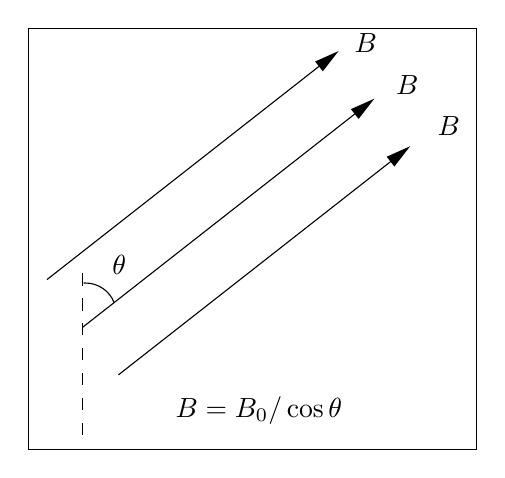
\begin{tikzpicture}[x=0.75pt,y=0.75pt,yscale=-1,xscale=1]
%uncomment if require: \path (0,750); %set diagram left start at 0, and has height of 750

%Straight Lines [id:da23592990358763366] 
\draw    (235,146.12) -- (373.94,37.23) ;
\draw [shift={(375.52,36)}, rotate = 501.92] [fill={rgb, 255:red, 0; green, 0; blue, 0 }  ][line width=0.08]  [draw opacity=0] (12,-3) -- (0,0) -- (12,3) -- cycle    ;
%Straight Lines [id:da026547845871476294] 
\draw    (252.24,169.06) -- (391.18,60.17) ;
\draw [shift={(392.76,58.94)}, rotate = 501.92] [fill={rgb, 255:red, 0; green, 0; blue, 0 }  ][line width=0.08]  [draw opacity=0] (12,-3) -- (0,0) -- (12,3) -- cycle    ;
%Straight Lines [id:da2785883781384344] 
\draw    (269.48,192) -- (408.43,83.12) ;
\draw [shift={(410,81.88)}, rotate = 501.92] [fill={rgb, 255:red, 0; green, 0; blue, 0 }  ][line width=0.08]  [draw opacity=0] (12,-3) -- (0,0) -- (12,3) -- cycle    ;
%Straight Lines [id:da35254547932852875] 
\draw  [dash pattern={on 4.5pt off 4.5pt}]  (252,143) -- (252,224) ;
%Shape: Arc [id:dp018362595446243413] 
\draw  [draw opacity=0] (252.68,147.77) .. controls (252.95,147.76) and (253.22,147.75) .. (253.5,147.75) .. controls (259.82,147.75) and (265.21,151.62) .. (267.31,157.07) -- (253.5,162.13) -- cycle ; \draw   (252.68,147.77) .. controls (252.95,147.76) and (253.22,147.75) .. (253.5,147.75) .. controls (259.82,147.75) and (265.21,151.62) .. (267.31,157.07) ;
%Shape: Rectangle [id:dp6795946491509408] 
\draw   (226,25) -- (442,25) -- (442,228) -- (226,228) -- cycle ;

% Text Node
\draw (265.25,133.15) node [anchor=north west][inner sep=0.75pt]    {$\theta $};
% Text Node
\draw (295.75,201.4) node [anchor=north west][inner sep=0.75pt]    {$B=B_{0} /\cos \theta $};
% Text Node
\draw (382,26.4) node [anchor=north west][inner sep=0.75pt]    {$B$};
% Text Node
\draw (402,46.4) node [anchor=north west][inner sep=0.75pt]    {$B$};
% Text Node
\draw (422,66.4) node [anchor=north west][inner sep=0.75pt]    {$B$};


\end{tikzpicture}

\end{center}
\end{center}
\end{solution}
\vspace{1cm}%\section{Problem 7}
\begin{problem}
Consider the given figure, the blue lines are perfectly reflecting hyperboloid mirrors with coincident foci shown in blue. A beam of light (red) is directed in through an opening at the top left of the system. Two observers $O_1$ and $O_2$ shall receive the light. Find the ratio of the energy density of the multiply reflected beam seen at $O_1$ to that at $O_2$.\\
$a) \quad 0$\\
$b) \quad 1/2$\\
$c) \quad 1$\\
$d) \quad 2$\\
\textbf{Note:} Neglect diffraction and other wave effects.
\begin{center}
    \definecolor{ffwwqq}{rgb}{1,0.4,0}
\definecolor{xdxdff}{rgb}{0.49019607843137253,0.49019607843137253,1}
\definecolor{ffqqqq}{rgb}{1,0,0}
\definecolor{qqqqff}{rgb}{0,0,1}
\begin{tikzpicture}[line cap=round,line join=round,>=triangle 45,x=1cm,y=1cm]
\begin{axis}[
x=1cm,y=1cm,
axis lines=middle,
ymajorgrids=true,
xmajorgrids=true,
xmin=-5.5348681371364865,
xmax=4.361500222676509,
ymin=-3.038270988144141,
ymax=4.96044323257081,
xtick={-4,-2,...,4},
ytick={-2,0,...,4},]
\clip(-5.5348681371364865,-3.038270988144141) rectangle (4.361500222676509,4.96044323257081);
\draw [samples=50,domain=-0.99:0.99,rotate around={0:(0,0)},xshift=0cm,yshift=0cm,line width=2pt,color=qqqqff] plot ({0.75*(1+(\x)^2)/(1-(\x)^2)},{0.565*2*(\x)/(1-(\x)^2)});
\draw [samples=50,domain=-0.99:0.99,rotate around={0:(0,0)},xshift=0cm,yshift=0cm,line width=2pt,color=qqqqff] plot ({0.75*(-1-(\x)^2)/(1-(\x)^2)},{0.565*(-2)*(\x)/(1-(\x)^2)});
\draw [samples=50,domain=-0.99:0.99,rotate around={0:(0,0)},xshift=0cm,yshift=0cm,line width=2pt,color=qqqqff] plot ({0.5*(1+(\x)^2)/(1-(\x)^2)},{0.865*2*(\x)/(1-(\x)^2)});
\draw [samples=50,domain=-0.99:0.99,rotate around={0:(0,0)},xshift=0cm,yshift=0cm,line width=2pt,color=qqqqff] plot ({0.5*(-1-(\x)^2)/(1-(\x)^2)},{0.865*(-2)*(\x)/(1-(\x)^2)});
\draw [->,line width=2.8pt,color=ffqqqq] (-3.857084611176678,4.081996066055657) -- (-3.0669647070714117,2.9531298337946326);
\draw [->,line width=2.8pt,color=ffqqqq] (-2.609314348408259,4.772247777142751) -- (-2.1224665620339076,3.3285532816392123);
\draw [line width=3.2pt,dash pattern=on 1pt off 1pt,color=ffwwqq] (-3.0669647070714117,2.9531298337946326)-- (-1,0);
\draw [line width=3.2pt,dash pattern=on 1pt off 1pt,color=ffwwqq] (-1,0)-- (-2.1224665620339076,3.3285532816392123);
\draw [->,line width=2.8pt,color=ffqqqq] (-3.4550340500135075,4.414219286214349) -- (-2.720067816314126,3.0927296215417623);
\draw [->,line width=2.8pt,color=ffqqqq] (-2.972519219091779,4.551647769246634) -- (-2.4218894093222323,3.281052825957698);
\begin{scriptsize}
\draw [fill=black] (-0.75,-0.5) circle (2pt);
\draw[color=black] (-0.14797896808363964,-0.26830809155726726) node {\textbf\Large{$O_1(-0.75,-0.5)$}};
\draw [fill=black] (-0.75,0.5) circle (2pt);
\draw[color=black] (-0.1887887345158581,0.7315311860321017) node {\textbf\Large{$O_2(-0.75,0.5)$}};
\draw [fill=xdxdff] (-1,0) circle (2.5pt);
\end{scriptsize}
\end{axis}
\end{tikzpicture}
\end{center}

\end{problem}
\begin{flushright}
\textbf{\Large{-Proposed by Hemansh Shah}}
\end{flushright}
\begin{solution}
Light rays going toward a focus of the hyperbola, upon reflection, change their paths so as to go through the other focus. Following the light path, we see that no rays can get to the point $O_1$.
\vspace{8mm}
\begin{center}
    

\tikzset{every picture/.style={line width=0.75pt}} %set default line width to 0.75pt        

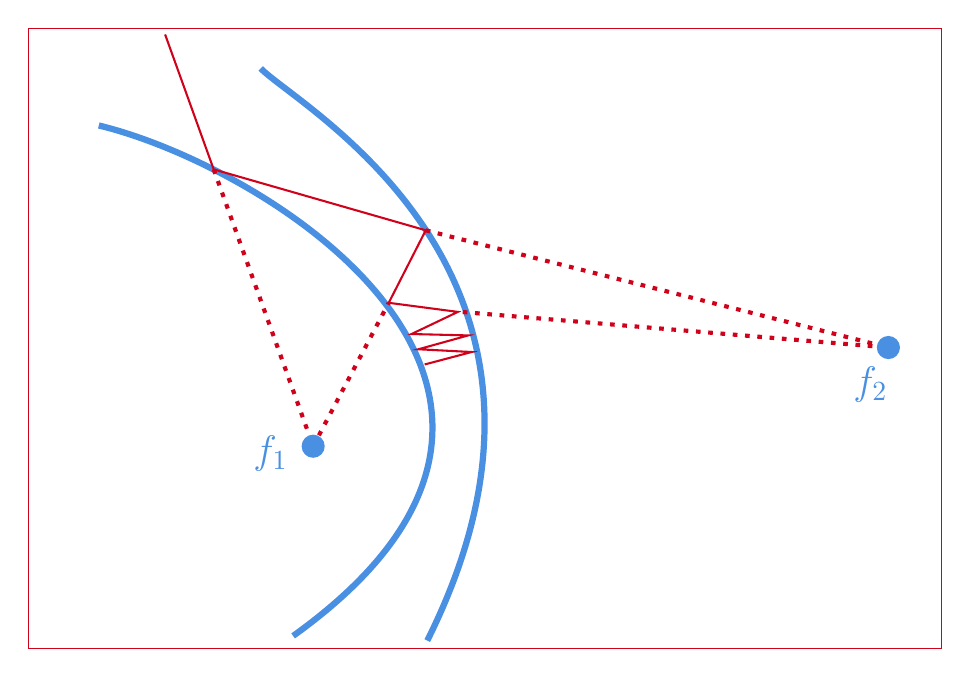
\begin{tikzpicture}[x=0.75pt,y=0.75pt,yscale=-1,xscale=1]
%uncomment if require: \path (0,750); %set diagram left start at 0, and has height of 750

%Curve Lines [id:da13594333926448599] 
\draw [color={rgb, 255:red, 74; green, 144; blue, 226 }  ,draw opacity=1 ][line width=2.25]    (135,67.84) .. controls (217.48,87.9) and (391.34,197.12) .. (228.62,313.78) ;
%Curve Lines [id:da043315931156913345] 
\draw [color={rgb, 255:red, 74; green, 144; blue, 226 }  ,draw opacity=1 ][line width=2.25]    (213.02,40.35) .. controls (230.85,58.92) and (381.68,139.17) .. (293.26,316.01) ;
%Straight Lines [id:da9885753190309774] 
\draw [color={rgb, 255:red, 208; green, 2; blue, 27 }  ,draw opacity=1 ][line width=0.75]    (166.95,24) -- (190.36,89.01) -- (292.52,118.36) -- (274.69,153.29) -- (308,157.67) -- (285.67,168.33) -- (313,169) -- (289,175.67) -- (314.67,177) -- (292,183) ;
%Straight Lines [id:da44875111196009176] 
\draw [color={rgb, 255:red, 208; green, 2; blue, 27 }  ,draw opacity=1 ][line width=1.5]  [dash pattern={on 1.69pt off 2.76pt}]  (292.52,118.36) -- (515.43,174.83) ;
%Straight Lines [id:da5427023462252292] 
\draw [color={rgb, 255:red, 208; green, 2; blue, 27 }  ,draw opacity=1 ][line width=1.5]  [dash pattern={on 1.69pt off 2.76pt}]  (310.35,157.74) -- (515.43,174.83) ;
%Straight Lines [id:da4399880157012206] 
\draw [color={rgb, 255:red, 208; green, 2; blue, 27 }  ,draw opacity=1 ][line width=1.5]  [dash pattern={on 1.69pt off 2.76pt}]  (190.36,89.01) -- (238.28,222.39) ;
%Straight Lines [id:da22821960507708172] 
\draw [color={rgb, 255:red, 208; green, 2; blue, 27 }  ,draw opacity=1 ][line width=1.5]  [dash pattern={on 1.69pt off 2.76pt}]  (238.28,222.39) -- (274.69,153.29) ;
%Shape: Ellipse [id:dp9694087247778784] 
\draw  [draw opacity=0][fill={rgb, 255:red, 74; green, 144; blue, 226 }  ,fill opacity=1 ] (232.71,222.39) .. controls (232.71,219.31) and (235.2,216.81) .. (238.28,216.81) .. controls (241.36,216.81) and (243.85,219.31) .. (243.85,222.39) .. controls (243.85,225.46) and (241.36,227.96) .. (238.28,227.96) .. controls (235.2,227.96) and (232.71,225.46) .. (232.71,222.39) -- cycle ;
%Shape: Circle [id:dp6089126920887125] 
\draw  [draw opacity=0][fill={rgb, 255:red, 74; green, 144; blue, 226 }  ,fill opacity=1 ] (509.85,174.83) .. controls (509.85,171.76) and (512.35,169.26) .. (515.43,169.26) .. controls (518.51,169.26) and (521,171.76) .. (521,174.83) .. controls (521,177.91) and (518.51,180.41) .. (515.43,180.41) .. controls (512.35,180.41) and (509.85,177.91) .. (509.85,174.83) -- cycle ;
%Shape: Rectangle [id:dp1627432962771942] 
\draw  [color={rgb, 255:red, 208; green, 2; blue, 27 }  ,draw opacity=1 ] (101,21) -- (541,21) -- (541,320) -- (101,320) -- cycle ;

% Text Node
\draw (208.19,216.22) node [anchor=north west][inner sep=0.75pt]  [font=\Large,color={rgb, 255:red, 74; green, 144; blue, 226 }  ,opacity=1 ]  {$f_{1}$};
% Text Node
\draw (497.23,182.78) node [anchor=north west][inner sep=0.75pt]  [font=\Large,color={rgb, 255:red, 74; green, 144; blue, 226 }  ,opacity=1 ]  {$f_{2}$};


\end{tikzpicture}

\end{center}
Hence, the answer is $0$.
\textbf{Answer: (a)}
\end{solution}
\vspace{1cm}%\section{Problem 8}
\begin{problem}
A disc of mass $M$, and radius $R$ is free to rotate about a fixed axis perpendicular to its surface and passing through its Centre of Mass. It is bound by a light spring, with a natural length of $L$. At its natural length, one end of the spring is connected to a fixed wall located at a distance of $L$ from the disc, and the other end is connected to the disc. The disc is rotated so that the spring forms a tangent to it and is released from that position. Samar sticks a ring of mass $16M$ and radius $R/N$ on the disc with the same fixed axis. He sticks this ring when the disc has maximum angular velocity and ensures he doesn't change its angular velocity. The spring snaps at a length $3\sqrt{L^2 + 2LR} - 2L$. You can assume that the spring exerts a force tangential to it at any given point. Friction is negligible everywhere. If $N\geq1$, find the minimum $N$ so the spring does not snap.
\vspace{6mm}
\begin{center}
    

\tikzset{every picture/.style={line width=0.75pt}} %set default line width to 0.75pt        

\begin{tikzpicture}[x=0.75pt,y=0.75pt,yscale=-1,xscale=1]
%uncomment if require: \path (0,537); %set diagram left start at 0, and has height of 537

%Straight Lines [id:da08727876157803438] 
\draw [line width=1.5]    (111,30) -- (518,30) ;
%Shape: Spring [id:dp23811323445365273] 
\draw   (328.32,40.9) .. controls (338.09,58.35) and (302.22,76.15) .. (296.84,66.55) .. controls (291.47,56.95) and (327.34,39.15) .. (337.12,56.6) .. controls (346.89,74.05) and (311.01,91.85) .. (305.64,82.26) .. controls (300.26,72.66) and (336.14,54.86) .. (345.91,72.31) .. controls (355.68,89.76) and (319.81,107.56) .. (314.43,97.96) .. controls (309.06,88.36) and (344.93,70.56) .. (354.71,88.01) .. controls (364.48,105.46) and (328.6,123.26) .. (323.23,113.67) .. controls (317.85,104.07) and (353.73,86.27) .. (363.5,103.72) .. controls (373.27,121.17) and (337.4,138.97) .. (332.02,129.37) .. controls (326.65,119.77) and (362.52,101.97) .. (372.3,119.42) .. controls (382.07,136.87) and (346.19,154.67) .. (340.82,145.08) .. controls (335.44,135.48) and (371.32,117.68) .. (381.09,135.13) .. controls (382.23,137.15) and (382.75,139.18) .. (382.77,141.17) ;
%Straight Lines [id:da6664577629638426] 
\draw    (324.6,31) -- (329,42.8) ;
%Straight Lines [id:da9213650211555284] 
\draw    (382.2,137.4) -- (394.6,217) ;
%Shape: Circle [id:dp9435150427604724] 
\draw   (204.2,258.1) .. controls (204.2,203.26) and (248.66,158.8) .. (303.5,158.8) .. controls (358.34,158.8) and (402.8,203.26) .. (402.8,258.1) .. controls (402.8,312.94) and (358.34,357.4) .. (303.5,357.4) .. controls (248.66,357.4) and (204.2,312.94) .. (204.2,258.1) -- cycle ;




\end{tikzpicture}

\end{center}
\end{problem}
\begin{flushright}
\textbf{\Large{-Proposed by Yash Bughani}}
\end{flushright}
\begin{solution}
Let elongation intitially = $X $= $\sqrt{L^2+2LR}-L$\\
Let maximum elongation  = $Y$ = $3\sqrt{L^2+2LR}-3L$\\
Let stiffness = k\\
$$\frac{kX^2}{2}=\frac{I}{2}\omega_{max}^2$$
$$\boxed{\omega_{max}=\sqrt{\frac{2k}{M}}\left(\frac{X}{R}\right)}$$
After placing ring:\\
$$\frac{kY^2}{2}=\frac{1}2{}\left(\frac{MR^2}{2}+\frac{16MR^2}{N^2}\right)\omega_{max}^2$$
$${kY^2}=MR^2\left(\frac{1}{2}+\frac{16}{N^2}\right)\left(\frac{2kX^2}{MR^2}\right)$$
$${Y^2}=\left(\frac{1}{2}+\frac{16}{N^2}\right)X^2$$
$$\frac{Y}{X}=\sqrt{1+\frac{32}{N^2}}$$
Substituting $Y$ and $X$:\\
$$\frac{3\sqrt{L^2+2LR}-3L}{{L^2+2LR}-L}=\sqrt{1+\frac{32}{N^2}} $$
$$\text{Hence }\boxed{N=2}$$
\end{solution}
\vspace{1cm}%\section{Problem 9}
\begin{problem}
A potential difference of $\displaystyle V{o}$ initiates the flow of steady current from top to bottom of the conductor (conductivity of medium is $\displaystyle \sigma $). Atharva broke the conductor and a hemispherical bump is generated in the conductor. Now he initiates the flow of current, he found that current flowing into that hemispherical bump of radius R is $\displaystyle k\pi \sigma R^{2}\frac{V{o}}{d}$ , Assuming $\displaystyle d\gg R$ find the value of $k$? 
\vspace{10mm}
\begin{center}
    

\tikzset{every picture/.style={line width=0.75pt}} %set default line width to 0.75pt        

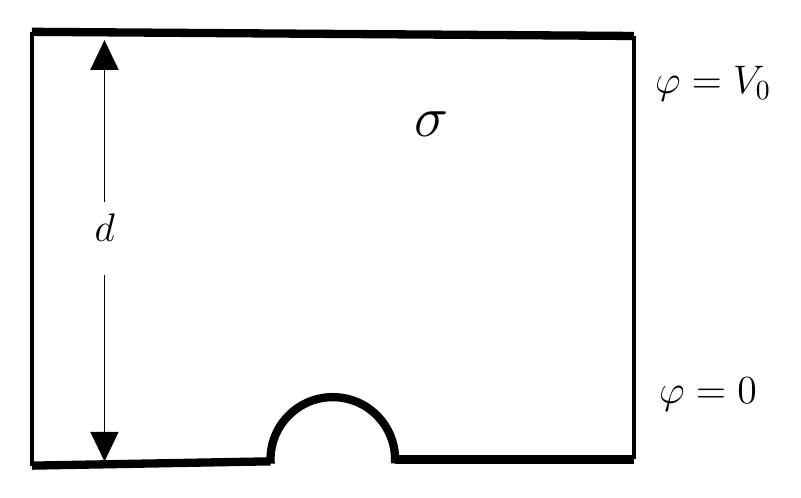
\begin{tikzpicture}[x=0.75pt,y=0.75pt,yscale=-1,xscale=1]
%uncomment if require: \path (0,537); %set diagram left start at 0, and has height of 537

%Straight Lines [id:da013965873027830922] 
\draw [line width=1.5]    (146,23) -- (146,232) ;
%Straight Lines [id:da26039574445576497] 
\draw [line width=1.5]    (436,25) -- (436,229) ;
%Straight Lines [id:da8920404489161631] 
\draw [line width=3]    (436,25) -- (146,23) ;
%Shape: Arc [id:dp740455878657255] 
\draw  [draw opacity=0][line width=3]  (261.07,231.07) .. controls (261.02,230.38) and (261,229.69) .. (261,229) .. controls (261,212.43) and (274.43,199) .. (291,199) .. controls (307.57,199) and (321,212.43) .. (321,229) .. controls (321,229.65) and (320.98,230.29) .. (320.94,230.93) -- (291,229) -- cycle ; \draw  [line width=3]  (261.07,231.07) .. controls (261.02,230.38) and (261,229.69) .. (261,229) .. controls (261,212.43) and (274.43,199) .. (291,199) .. controls (307.57,199) and (321,212.43) .. (321,229) .. controls (321,229.65) and (320.98,230.29) .. (320.94,230.93) ;
%Straight Lines [id:da3028129433938429] 
\draw [line width=3]    (261.01,229.94) -- (146,232) ;
%Straight Lines [id:da5385350556293031] 
\draw [line width=3]    (436,229) -- (321,229) ;

%Straight Lines [id:da11953546043815222] 
\draw    (181,105) -- (181,30) ;
\draw [shift={(181,27)}, rotate = 450] [fill={rgb, 255:red, 0; green, 0; blue, 0 }  ][line width=0.08]  [draw opacity=0] (14.29,-6.86) -- (0,0) -- (14.29,6.86) -- cycle    ;
%Straight Lines [id:da04514608560286959] 
\draw    (181,140) -- (181,227) ;
\draw [shift={(181,230)}, rotate = 270] [fill={rgb, 255:red, 0; green, 0; blue, 0 }  ][line width=0.08]  [draw opacity=0] (14.29,-6.86) -- (0,0) -- (14.29,6.86) -- cycle    ;

% Text Node
\draw (175,109.4) node [anchor=north west][inner sep=0.75pt]  [font=\Large]  {$d$};
% Text Node
\draw (329,60.4) node [anchor=north west][inner sep=0.75pt]  [font=\huge]  {$\sigma $};
% Text Node
\draw (445,38.4) node [anchor=north west][inner sep=0.75pt]  [font=\Large]  {$\varphi =V_{0}$};
% Text Node
\draw (447,188.4) node [anchor=north west][inner sep=0.75pt]  [font=\Large]  {$\varphi =0$};


\end{tikzpicture}

\end{center}
\end{problem}
\begin{flushright}
\textbf{\Large{-Proposed by Harshit Gupta}}
\end{flushright}
\begin{solution}

Since $R<<d$, $\vec{E}$ everywhere except near hemisphere will be:
$$
\boxed{
    |\vec{E}|=\frac{V_0}{d}
}
$$
\begin{center}
    

\tikzset{every picture/.style={line width=0.75pt}} %set default line width to 0.75pt        

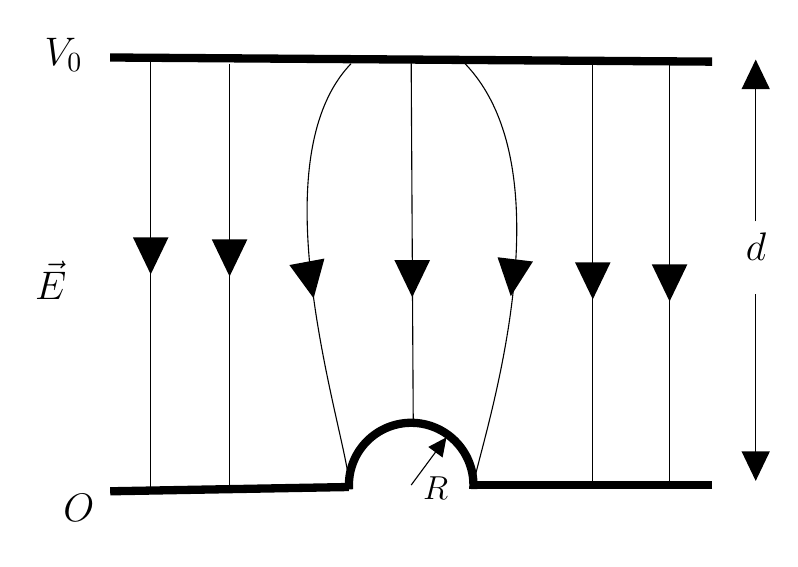
\begin{tikzpicture}[x=0.75pt,y=0.75pt,yscale=-1,xscale=1]
%uncomment if require: \path (0,537); %set diagram left start at 0, and has height of 537

%Straight Lines [id:da624999585450982] 
\draw [line width=3]    (436,25) -- (146,23) ;
%Shape: Arc [id:dp37178586221495746] 
\draw  [draw opacity=0][line width=3]  (261.07,231.07) .. controls (261.02,230.38) and (261,229.69) .. (261,229) .. controls (261,212.43) and (274.43,199) .. (291,199) .. controls (307.57,199) and (321,212.43) .. (321,229) .. controls (321,229.65) and (320.98,230.29) .. (320.94,230.93) -- (291,229) -- cycle ; \draw  [line width=3]  (261.07,231.07) .. controls (261.02,230.38) and (261,229.69) .. (261,229) .. controls (261,212.43) and (274.43,199) .. (291,199) .. controls (307.57,199) and (321,212.43) .. (321,229) .. controls (321,229.65) and (320.98,230.29) .. (320.94,230.93) ;
%Straight Lines [id:da96775558191455] 
\draw [line width=3]    (261.01,229.94) -- (146,232) ;
%Straight Lines [id:da29120956460143366] 
\draw [line width=3]    (436,229) -- (321,229) ;
%Straight Lines [id:da11953546043815222] 
\draw    (457,102) -- (457,27) ;
\draw [shift={(457,24)}, rotate = 450] [fill={rgb, 255:red, 0; green, 0; blue, 0 }  ][line width=0.08]  [draw opacity=0] (14.29,-6.86) -- (0,0) -- (14.29,6.86) -- cycle    ;
%Straight Lines [id:da04514608560286959] 
\draw    (457,137) -- (457,224) ;
\draw [shift={(457,227)}, rotate = 270] [fill={rgb, 255:red, 0; green, 0; blue, 0 }  ][line width=0.08]  [draw opacity=0] (14.29,-6.86) -- (0,0) -- (14.29,6.86) -- cycle    ;
%Curve Lines [id:da02086193112392154] 
\draw    (321,229) .. controls (323,213) and (370,79) .. (316,25) ;
%Curve Lines [id:da7273542230497207] 
\draw    (261.01,229.94) .. controls (263.01,213.94) and (214,76) .. (262,26) ;
%Straight Lines [id:da46922008941212745] 
\draw    (291,24) -- (292,199) ;
%Straight Lines [id:da3238455563720479] 
\draw    (203.51,26) -- (203.51,230.97) ;
%Straight Lines [id:da6457138806437486] 
\draw    (378.5,24.03) -- (378.5,229) ;
%Straight Lines [id:da8123242047480104] 
\draw    (415.5,25.03) -- (415.5,230) ;
%Straight Lines [id:da06625446492368203] 
\draw    (165.51,25) -- (165.51,229.97) ;
%Straight Lines [id:da47895872621748037] 
\draw    (291,229) -- (306.22,208.41) ;
\draw [shift={(308,206)}, rotate = 486.47] [fill={rgb, 255:red, 0; green, 0; blue, 0 }  ][line width=0.08]  [draw opacity=0] (8.93,-4.29) -- (0,0) -- (8.93,4.29) -- cycle    ;
%Straight Lines [id:da18879475422962377] 
\draw    (165.51,114.48) -- (165.51,124.48) ;
\draw [shift={(165.51,127.48)}, rotate = 270] [fill={rgb, 255:red, 0; green, 0; blue, 0 }  ][line width=0.08]  [draw opacity=0] (17.86,-8.58) -- (0,0) -- (17.86,8.58) -- cycle    ;
%Straight Lines [id:da7680075968925193] 
\draw    (203.51,115.48) -- (203.51,125.48) ;
\draw [shift={(203.51,128.48)}, rotate = 270] [fill={rgb, 255:red, 0; green, 0; blue, 0 }  ][line width=0.08]  [draw opacity=0] (17.86,-8.58) -- (0,0) -- (17.86,8.58) -- cycle    ;
%Straight Lines [id:da4255762753428194] 
\draw    (241.51,125.48) -- (243.46,136.05) ;
\draw [shift={(244,139)}, rotate = 259.55] [fill={rgb, 255:red, 0; green, 0; blue, 0 }  ][line width=0.08]  [draw opacity=0] (17.86,-8.58) -- (0,0) -- (17.86,8.58) -- cycle    ;
%Straight Lines [id:da9148139031356599] 
\draw    (291.51,125.48) -- (291.51,135.48) ;
\draw [shift={(291.51,138.48)}, rotate = 270] [fill={rgb, 255:red, 0; green, 0; blue, 0 }  ][line width=0.08]  [draw opacity=0] (17.86,-8.58) -- (0,0) -- (17.86,8.58) -- cycle    ;
%Straight Lines [id:da5745730716981676] 
\draw    (340.51,125.48) -- (339.36,135.02) ;
\draw [shift={(339,138)}, rotate = 276.87] [fill={rgb, 255:red, 0; green, 0; blue, 0 }  ][line width=0.08]  [draw opacity=0] (17.86,-8.58) -- (0,0) -- (17.86,8.58) -- cycle    ;
%Straight Lines [id:da728165215851676] 
\draw    (415.5,127.52) -- (415.5,137.52) ;
\draw [shift={(415.5,140.52)}, rotate = 270] [fill={rgb, 255:red, 0; green, 0; blue, 0 }  ][line width=0.08]  [draw opacity=0] (17.86,-8.58) -- (0,0) -- (17.86,8.58) -- cycle    ;
%Straight Lines [id:da5506489652289128] 
\draw    (378.5,126.52) -- (378.5,136.52) ;
\draw [shift={(378.5,139.52)}, rotate = 270] [fill={rgb, 255:red, 0; green, 0; blue, 0 }  ][line width=0.08]  [draw opacity=0] (17.86,-8.58) -- (0,0) -- (17.86,8.58) -- cycle    ;

% Text Node
\draw (451,106.4) node [anchor=north west][inner sep=0.75pt]  [font=\Large]  {$d$};
% Text Node
\draw (295.5,223.9) node [anchor=north west][inner sep=0.75pt]  [font=\large]  {$R$};
% Text Node
\draw (108.5,119.9) node [anchor=north west][inner sep=0.75pt]  [font=\Large]  {$\vec{E}$};
% Text Node
\draw (106.5,8.9) node [anchor=north west][inner sep=0.75pt]  [font=\Large]  {$ \begin{array}{l}
V_{0}\\
\end{array}$};
% Text Node
\draw (115.5,228.4) node [anchor=north west][inner sep=0.75pt]  [font=\Large]  {$ \begin{array}{l}
O\\
\end{array}$};


\end{tikzpicture}

\end{center}
In uniform electric field grounded sphere gets polarised with dipole moment:


\begin{center}
    
\tikzset{every picture/.style={line width=0.75pt}} %set default line width to 0.75pt        

\begin{tikzpicture}[x=0.75pt,y=0.75pt,yscale=-1,xscale=1]
%uncomment if require: \path (0,391); %set diagram left start at 0, and has height of 391

%Shape: Circle [id:dp5981522343068211] 
\draw   (273,184.4) .. controls (273,167.06) and (287.06,153) .. (304.4,153) .. controls (321.74,153) and (335.8,167.06) .. (335.8,184.4) .. controls (335.8,201.74) and (321.74,215.8) .. (304.4,215.8) .. controls (287.06,215.8) and (273,201.74) .. (273,184.4) -- cycle ;
%Curve Lines [id:da575968783666897] 
\draw    (239.8,48.2) .. controls (244.8,76.2) and (251.8,134.2) .. (283.8,160.2) ;
\draw [shift={(252.86,108.77)}, rotate = 253.03] [color={rgb, 255:red, 0; green, 0; blue, 0 }  ][line width=0.75]    (10.93,-4.9) .. controls (6.95,-2.3) and (3.31,-0.67) .. (0,0) .. controls (3.31,0.67) and (6.95,2.3) .. (10.93,4.9)   ;
%Straight Lines [id:da12110805903894772] 
\draw    (303.8,41.2) -- (304.4,153) ;
\draw [shift={(304.1,97.1)}, rotate = 269.69] [color={rgb, 255:red, 0; green, 0; blue, 0 }  ][line width=0.75]    (10.93,-4.9) .. controls (6.95,-2.3) and (3.31,-0.67) .. (0,0) .. controls (3.31,0.67) and (6.95,2.3) .. (10.93,4.9)   ;
%Curve Lines [id:da08990593309278783] 
\draw    (360.8,44.2) .. controls (360.8,84.2) and (350.8,141.2) .. (323.8,160.2) ;
\draw [shift={(353.28,106.81)}, rotate = 283.37] [color={rgb, 255:red, 0; green, 0; blue, 0 }  ][line width=0.75]    (10.93,-4.9) .. controls (6.95,-2.3) and (3.31,-0.67) .. (0,0) .. controls (3.31,0.67) and (6.95,2.3) .. (10.93,4.9)   ;
%Straight Lines [id:da5994163919336195] 
\draw    (304.4,215.8) -- (305.8,326.2) ;
\draw [shift={(305.1,271)}, rotate = 89.27] [color={rgb, 255:red, 0; green, 0; blue, 0 }  ][line width=0.75]    (10.93,-4.9) .. controls (6.95,-2.3) and (3.31,-0.67) .. (0,0) .. controls (3.31,0.67) and (6.95,2.3) .. (10.93,4.9)   ;
%Curve Lines [id:da9633174082102978] 
\draw    (249.8,320.2) .. controls (249.8,278.2) and (257.8,238.2) .. (282.8,207.2) ;
\draw [shift={(256.77,260.15)}, rotate = 463.76] [color={rgb, 255:red, 0; green, 0; blue, 0 }  ][line width=0.75]    (10.93,-4.9) .. controls (6.95,-2.3) and (3.31,-0.67) .. (0,0) .. controls (3.31,0.67) and (6.95,2.3) .. (10.93,4.9)   ;
%Curve Lines [id:da9296454542832435] 
\draw    (322.8,210.2) .. controls (361.8,242.2) and (362.8,284.2) .. (361.8,320.2) ;
\draw [shift={(356.35,260.29)}, rotate = 71.92] [color={rgb, 255:red, 0; green, 0; blue, 0 }  ][line width=0.75]    (10.93,-4.9) .. controls (6.95,-2.3) and (3.31,-0.67) .. (0,0) .. controls (3.31,0.67) and (6.95,2.3) .. (10.93,4.9)   ;
%Straight Lines [id:da1901626360219637] 
\draw    (304.4,172.4) -- (304.4,194.4) ;
\draw [shift={(304.4,196.4)}, rotate = 270] [color={rgb, 255:red, 0; green, 0; blue, 0 }  ][line width=0.75]    (10.93,-3.29) .. controls (6.95,-1.4) and (3.31,-0.3) .. (0,0) .. controls (3.31,0.3) and (6.95,1.4) .. (10.93,3.29)   ;
%Shape: Right Angle [id:dp14993923421261757] 
\draw   (336,179) -- (372.8,179) -- (372.8,236.2) ;
%Straight Lines [id:da5946517817217605] 
\draw    (356.4,236.1) -- (389.2,236.3) ;
%Straight Lines [id:da03468270838961174] 
\draw    (365,242) -- (380.8,242.2) ;
%Straight Lines [id:da2715511184321706] 
\draw    (368,247) -- (377.8,247.2) ;
%Straight Lines [id:da43816073822045] 
\draw    (157.8,81.2) -- (157.8,281.2) ;
\draw [shift={(157.8,181.2)}, rotate = 270] [color={rgb, 255:red, 0; green, 0; blue, 0 }  ][line width=0.75]    (10.93,-4.9) .. controls (6.95,-2.3) and (3.31,-0.67) .. (0,0) .. controls (3.31,0.67) and (6.95,2.3) .. (10.93,4.9)   ;
%Straight Lines [id:da8773884473619051] 
\draw    (452.8,80.2) -- (452.8,280.2) ;
\draw [shift={(452.8,180.2)}, rotate = 270] [color={rgb, 255:red, 0; green, 0; blue, 0 }  ][line width=0.75]    (10.93,-4.9) .. controls (6.95,-2.3) and (3.31,-0.67) .. (0,0) .. controls (3.31,0.67) and (6.95,2.3) .. (10.93,4.9)   ;

% Text Node
\draw (312.4,174.8) node [anchor=north west][inner sep=0.75pt]  [font=\footnotesize]  {$\vec{p}$};
% Text Node
\draw (310,161) node [anchor=north west][inner sep=0.75pt]   [align=left] {\mbox{-}};
% Text Node
\draw (298.4,155) node [anchor=north west][inner sep=0.75pt]   [align=left] {\mbox{-}};
% Text Node
\draw (286.8,158.2) node [anchor=north west][inner sep=0.75pt]   [align=left] {\mbox{-}};
% Text Node
\draw (294,164) node [anchor=north west][inner sep=0.75pt]   [align=left] {\mbox{-}};
% Text Node
\draw (322,159) node [anchor=north west][inner sep=0.75pt]   [align=left] {\mbox{-}};
% Text Node
\draw (300,198) node [anchor=north west][inner sep=0.75pt]   [align=left] {+};
% Text Node
\draw (290,192) node [anchor=north west][inner sep=0.75pt]   [align=left] {+};
% Text Node
\draw (311,193) node [anchor=north west][inner sep=0.75pt]   [align=left] {+};
% Text Node
\draw (280,186.4) node [anchor=north west][inner sep=0.75pt]   [align=left] {+};
% Text Node
\draw (116,136.4) node [anchor=north west][inner sep=0.75pt]    {$E_{0}$};


\end{tikzpicture}
\end{center}

$$
\boxed{
    | \vec{p} |=\frac{4}{3} \pi R^3 3\epsilon_0 \vec{E_0}
}
$$


So, surface charge density will be:


\begin{center}
    

\tikzset{every picture/.style={line width=0.75pt}} %set default line width to 0.75pt        

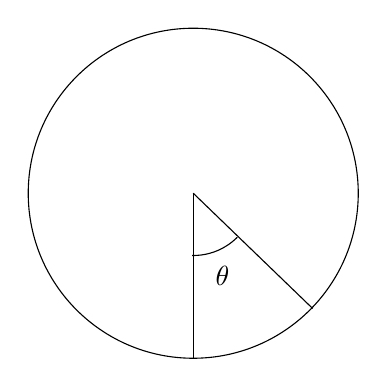
\begin{tikzpicture}[x=0.75pt,y=0.75pt,yscale=-1,xscale=1]
%uncomment if require: \path (0,445); %set diagram left start at 0, and has height of 445

%Shape: Circle [id:dp29550676628585726] 
\draw   (254,129.5) .. controls (254,85.59) and (289.59,50) .. (333.5,50) .. controls (377.41,50) and (413,85.59) .. (413,129.5) .. controls (413,173.41) and (377.41,209) .. (333.5,209) .. controls (289.59,209) and (254,173.41) .. (254,129.5) -- cycle ;
%Straight Lines [id:da6222823525744394] 
\draw    (333.5,129.5) -- (333.5,209) ;
%Straight Lines [id:da9652099390491349] 
\draw    (333.5,129.5) -- (391,185) ;
%Shape: Arc [id:dp40168092509805575] 
\draw  [draw opacity=0] (354.72,150.71) .. controls (353.26,152.17) and (351.62,153.51) .. (349.81,154.68) .. controls (344.61,158.05) and (338.75,159.6) .. (332.99,159.5) -- (333.5,129.5) -- cycle ; \draw   (354.72,150.71) .. controls (353.26,152.17) and (351.62,153.51) .. (349.81,154.68) .. controls (344.61,158.05) and (338.75,159.6) .. (332.99,159.5) ;

% Text Node
\draw (343,163.4) node [anchor=north west][inner sep=0.75pt]    {$\theta $};


\end{tikzpicture}

\end{center}


$$\boxed{
\sigma = -3\epsilon_0 E_0 cos\theta
}
$$


\begin{center}
    

\tikzset{every picture/.style={line width=0.75pt}} %set default line width to 0.75pt        

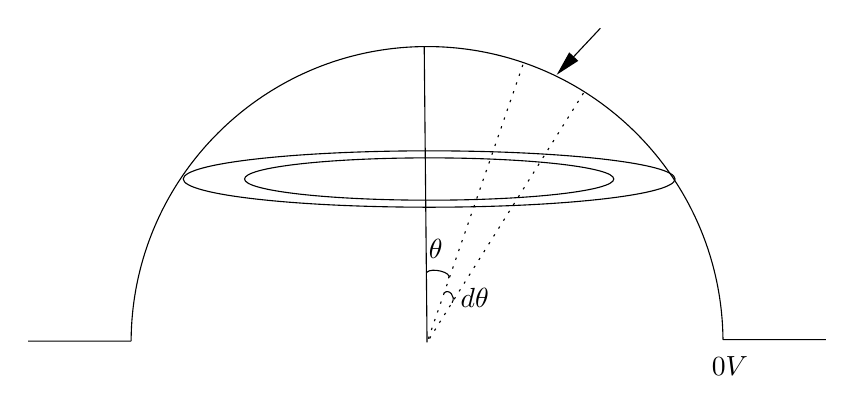
\begin{tikzpicture}[x=0.75pt,y=0.75pt,yscale=-1,xscale=1]
%uncomment if require: \path (0,445); %set diagram left start at 0, and has height of 445

%Shape: Arc [id:dp7092955729857724] 
\draw  [draw opacity=0] (86.57,186.74) .. controls (86.93,108.3) and (150.63,44.83) .. (229.15,44.83) .. controls (307.44,44.83) and (371,107.93) .. (371.73,186.04) -- (229.15,187.41) -- cycle ; \draw   (86.57,186.74) .. controls (86.93,108.3) and (150.63,44.83) .. (229.15,44.83) .. controls (307.44,44.83) and (371,107.93) .. (371.73,186.04) ;
%Shape: Ellipse [id:dp8602810270275838] 
\draw   (111.69,108.65) .. controls (111.69,101.15) and (164.73,95.07) .. (230.17,95.07) .. controls (295.61,95.07) and (348.65,101.15) .. (348.65,108.65) .. controls (348.65,116.15) and (295.61,122.23) .. (230.17,122.23) .. controls (164.73,122.23) and (111.69,116.15) .. (111.69,108.65) -- cycle ;
%Shape: Ellipse [id:dp08885150246677687] 
\draw   (141.22,108.65) .. controls (141.22,103.02) and (181.05,98.46) .. (230.17,98.46) .. controls (279.29,98.46) and (319.12,103.02) .. (319.12,108.65) .. controls (319.12,114.28) and (279.29,118.85) .. (230.17,118.85) .. controls (181.05,118.85) and (141.22,114.28) .. (141.22,108.65) -- cycle ;
%Straight Lines [id:da7888989400947082] 
\draw    (227.79,44.83) -- (229.15,187.41) ;
%Straight Lines [id:da22547779818918556] 
\draw  [dash pattern={on 0.84pt off 2.51pt}]  (304.52,67.23) -- (229.15,187.41) ;
%Straight Lines [id:da16034688721639645] 
\draw  [dash pattern={on 0.84pt off 2.51pt}]  (275.32,53.65) -- (229.15,187.41) ;
%Curve Lines [id:da849779096762004] 
\draw    (237.3,163.65) .. controls (239.51,161.1) and (243.24,165.35) .. (241.2,168.23) ;
%Curve Lines [id:da5957472202509568] 
\draw    (228.98,153.63) .. controls (231.19,151.09) and (241.54,153.63) .. (239.51,156.52) ;
%Straight Lines [id:da9285834942191944] 
\draw    (312.67,36) -- (292.99,56.95) ;
\draw [shift={(291.62,58.41)}, rotate = 313.21000000000004] [fill={rgb, 255:red, 0; green, 0; blue, 0 }  ][line width=0.08]  [draw opacity=0] (12,-3) -- (0,0) -- (12,3) -- cycle    ;
%Straight Lines [id:da3876261754139352] 
\draw    (37,186.73) -- (86.57,186.74) ;
%Straight Lines [id:da7100257608791913] 
\draw    (371.73,186.04) -- (421.3,186.05) ;

% Text Node
\draw (244.11,159.95) node [anchor=north west][inner sep=0.75pt]    {$d\theta $};
% Text Node
\draw (228.75,136.36) node [anchor=north west][inner sep=0.75pt]    {$\theta $};
% Text Node
\draw (365.11,192.95) node [anchor=north west][inner sep=0.75pt]    {$0V$};


\end{tikzpicture}

\end{center}


$$\boxed{\vec{E} = \frac{\sigma}{\epsilon_0}=-3E_0 cos\theta \hat{r}} $$

Ohms law:

$$\vec{J}=\sigma \vec{E}$$
$$\vec{J} = -3E_0 \cos \theta \sigma \hat{r}$$
$$\ \ \ = -3\sigma \cos\theta\frac{V_0}{d} \hat{r}$$

So, total current flowing inside hemisphere will be 
$$ I= \int \vec{J} \cdot d \vec{A}$$
$$\ \ \ = \int_0^{\frac{\pi}{2}} 3\sigma \cos\theta\frac{V_0}{d} \cdot 2\pi R \sin \theta R d \theta$$

$$\boxed{\text{Hence, Answer=} \frac{3\pi R^2 \sigma V_0}{d}}$$
 
\textbf{Answer: 3}

\end{solution}

\vspace{1cm}%\section{Problem 10}
\begin{problem}

Samar and Aayush live in a strange magical world. For doing magic, they need a perfect cylindrical wand. Samar and Aayush are sworn enemies and in a previous fight between them, Samar's wand broke so he made a new wand. He intended to make a perfect wand, but while using the charm ``Rictumsempra", Aayush disturbed him and as a result, the radius of Samar's wand became:

$R(x)=R_0+r\sin^2 \frac{2 \pi x}{a}$ \ and length of the wand is $\ell$.

Somehow this wand reached Aditya in the Muggle world and Aditya wanted to calculate the resistance of the wand. He found the resistivity of the wand's material to be $\rho$. Determine the resistance of the wand that Aditya found. 
Assume that $r\ll R$ and $a\ll l$
\vspace{5mm}

\textbf{a)}The resistance of wand determined by Aditya will be $\frac{\rho l}{\pi R_o^2}$ \newline 
\textbf{b)}The resistance of wand determined by Aditya will be $\frac{\rho l}{\pi R_o^2}\qty(1+\frac{r^2}{R_o^2})$ 
\newline \textbf{c)}The resistance of wand determined by Aditya will be $\frac{\rho l}{\pi R_o^2}\qty(1-\frac{r^2}{R_o^2})$ 
\newline \textbf{d)}The resistance of wand determined by Aditya will be $\frac{\rho l}{\pi R_o^2}\qty(1-\frac{r}{R_o})$
\vspace{10mm}
\begin{center}
    

\tikzset{every picture/.style={line width=0.75pt}} %set default line width to 0.75pt        

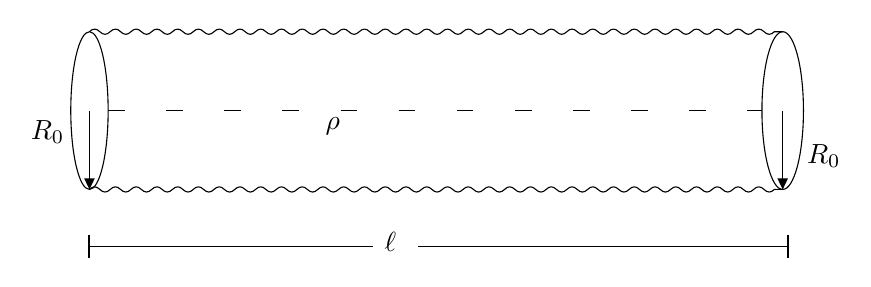
\begin{tikzpicture}[x=0.75pt,y=0.75pt,yscale=-1,xscale=1]
%uncomment if require: \path (0,448); %set diagram left start at 0, and has height of 448

%Shape: Ellipse [id:dp3730606810567325] 
\draw   (95.5,170) .. controls (95.5,149.01) and (99.53,132) .. (104.5,132) .. controls (109.47,132) and (113.5,149.01) .. (113.5,170) .. controls (113.5,190.99) and (109.47,208) .. (104.5,208) .. controls (99.53,208) and (95.5,190.99) .. (95.5,170) -- cycle ;
%Shape: Ellipse [id:dp6366590494916369] 
\draw   (428.5,170) .. controls (428.5,149.01) and (432.98,132) .. (438.5,132) .. controls (444.02,132) and (448.5,149.01) .. (448.5,170) .. controls (448.5,190.99) and (444.02,208) .. (438.5,208) .. controls (432.98,208) and (428.5,190.99) .. (428.5,170) -- cycle ;
%Straight Lines [id:da17407338648740622] 
\draw    (104.5,132) .. controls (106.17,130.33) and (107.83,130.33) .. (109.5,132) .. controls (111.17,133.67) and (112.83,133.67) .. (114.5,132) .. controls (116.17,130.33) and (117.83,130.33) .. (119.5,132) .. controls (121.17,133.67) and (122.83,133.67) .. (124.5,132) .. controls (126.17,130.33) and (127.83,130.33) .. (129.5,132) .. controls (131.17,133.67) and (132.83,133.67) .. (134.5,132) .. controls (136.17,130.33) and (137.83,130.33) .. (139.5,132) .. controls (141.17,133.67) and (142.83,133.67) .. (144.5,132) .. controls (146.17,130.33) and (147.83,130.33) .. (149.5,132) .. controls (151.17,133.67) and (152.83,133.67) .. (154.5,132) .. controls (156.17,130.33) and (157.83,130.33) .. (159.5,132) .. controls (161.17,133.67) and (162.83,133.67) .. (164.5,132) .. controls (166.17,130.33) and (167.83,130.33) .. (169.5,132) .. controls (171.17,133.67) and (172.83,133.67) .. (174.5,132) .. controls (176.17,130.33) and (177.83,130.33) .. (179.5,132) .. controls (181.17,133.67) and (182.83,133.67) .. (184.5,132) .. controls (186.17,130.33) and (187.83,130.33) .. (189.5,132) .. controls (191.17,133.67) and (192.83,133.67) .. (194.5,132) .. controls (196.17,130.33) and (197.83,130.33) .. (199.5,132) .. controls (201.17,133.67) and (202.83,133.67) .. (204.5,132) .. controls (206.17,130.33) and (207.83,130.33) .. (209.5,132) .. controls (211.17,133.67) and (212.83,133.67) .. (214.5,132) .. controls (216.17,130.33) and (217.83,130.33) .. (219.5,132) .. controls (221.17,133.67) and (222.83,133.67) .. (224.5,132) .. controls (226.17,130.33) and (227.83,130.33) .. (229.5,132) .. controls (231.17,133.67) and (232.83,133.67) .. (234.5,132) .. controls (236.17,130.33) and (237.83,130.33) .. (239.5,132) .. controls (241.17,133.67) and (242.83,133.67) .. (244.5,132) .. controls (246.17,130.33) and (247.83,130.33) .. (249.5,132) .. controls (251.17,133.67) and (252.83,133.67) .. (254.5,132) .. controls (256.17,130.33) and (257.83,130.33) .. (259.5,132) .. controls (261.17,133.67) and (262.83,133.67) .. (264.5,132) .. controls (266.17,130.33) and (267.83,130.33) .. (269.5,132) .. controls (271.17,133.67) and (272.83,133.67) .. (274.5,132) .. controls (276.17,130.33) and (277.83,130.33) .. (279.5,132) .. controls (281.17,133.67) and (282.83,133.67) .. (284.5,132) .. controls (286.17,130.33) and (287.83,130.33) .. (289.5,132) .. controls (291.17,133.67) and (292.83,133.67) .. (294.5,132) .. controls (296.17,130.33) and (297.83,130.33) .. (299.5,132) .. controls (301.17,133.67) and (302.83,133.67) .. (304.5,132) .. controls (306.17,130.33) and (307.83,130.33) .. (309.5,132) .. controls (311.17,133.67) and (312.83,133.67) .. (314.5,132) .. controls (316.17,130.33) and (317.83,130.33) .. (319.5,132) .. controls (321.17,133.67) and (322.83,133.67) .. (324.5,132) .. controls (326.17,130.33) and (327.83,130.33) .. (329.5,132) .. controls (331.17,133.67) and (332.83,133.67) .. (334.5,132) .. controls (336.17,130.33) and (337.83,130.33) .. (339.5,132) .. controls (341.17,133.67) and (342.83,133.67) .. (344.5,132) .. controls (346.17,130.33) and (347.83,130.33) .. (349.5,132) .. controls (351.17,133.67) and (352.83,133.67) .. (354.5,132) .. controls (356.17,130.33) and (357.83,130.33) .. (359.5,132) .. controls (361.17,133.67) and (362.83,133.67) .. (364.5,132) .. controls (366.17,130.33) and (367.83,130.33) .. (369.5,132) .. controls (371.17,133.67) and (372.83,133.67) .. (374.5,132) .. controls (376.17,130.33) and (377.83,130.33) .. (379.5,132) .. controls (381.17,133.67) and (382.83,133.67) .. (384.5,132) .. controls (386.17,130.33) and (387.83,130.33) .. (389.5,132) .. controls (391.17,133.67) and (392.83,133.67) .. (394.5,132) .. controls (396.17,130.33) and (397.83,130.33) .. (399.5,132) .. controls (401.17,133.67) and (402.83,133.67) .. (404.5,132) .. controls (406.17,130.33) and (407.83,130.33) .. (409.5,132) .. controls (411.17,133.67) and (412.83,133.67) .. (414.5,132) .. controls (416.17,130.33) and (417.83,130.33) .. (419.5,132) .. controls (421.17,133.67) and (422.83,133.67) .. (424.5,132) .. controls (426.17,130.33) and (427.83,130.33) .. (429.5,132) .. controls (431.17,133.67) and (432.83,133.67) .. (434.5,132) -- (438.5,132) -- (438.5,132) ;
%Straight Lines [id:da41974809031947014] 
\draw    (104.5,208) .. controls (106.17,206.33) and (107.83,206.33) .. (109.5,208) .. controls (111.17,209.67) and (112.83,209.67) .. (114.5,208) .. controls (116.17,206.33) and (117.83,206.33) .. (119.5,208) .. controls (121.17,209.67) and (122.83,209.67) .. (124.5,208) .. controls (126.17,206.33) and (127.83,206.33) .. (129.5,208) .. controls (131.17,209.67) and (132.83,209.67) .. (134.5,208) .. controls (136.17,206.33) and (137.83,206.33) .. (139.5,208) .. controls (141.17,209.67) and (142.83,209.67) .. (144.5,208) .. controls (146.17,206.33) and (147.83,206.33) .. (149.5,208) .. controls (151.17,209.67) and (152.83,209.67) .. (154.5,208) .. controls (156.17,206.33) and (157.83,206.33) .. (159.5,208) .. controls (161.17,209.67) and (162.83,209.67) .. (164.5,208) .. controls (166.17,206.33) and (167.83,206.33) .. (169.5,208) .. controls (171.17,209.67) and (172.83,209.67) .. (174.5,208) .. controls (176.17,206.33) and (177.83,206.33) .. (179.5,208) .. controls (181.17,209.67) and (182.83,209.67) .. (184.5,208) .. controls (186.17,206.33) and (187.83,206.33) .. (189.5,208) .. controls (191.17,209.67) and (192.83,209.67) .. (194.5,208) .. controls (196.17,206.33) and (197.83,206.33) .. (199.5,208) .. controls (201.17,209.67) and (202.83,209.67) .. (204.5,208) .. controls (206.17,206.33) and (207.83,206.33) .. (209.5,208) .. controls (211.17,209.67) and (212.83,209.67) .. (214.5,208) .. controls (216.17,206.33) and (217.83,206.33) .. (219.5,208) .. controls (221.17,209.67) and (222.83,209.67) .. (224.5,208) .. controls (226.17,206.33) and (227.83,206.33) .. (229.5,208) .. controls (231.17,209.67) and (232.83,209.67) .. (234.5,208) .. controls (236.17,206.33) and (237.83,206.33) .. (239.5,208) .. controls (241.17,209.67) and (242.83,209.67) .. (244.5,208) .. controls (246.17,206.33) and (247.83,206.33) .. (249.5,208) .. controls (251.17,209.67) and (252.83,209.67) .. (254.5,208) .. controls (256.17,206.33) and (257.83,206.33) .. (259.5,208) .. controls (261.17,209.67) and (262.83,209.67) .. (264.5,208) .. controls (266.17,206.33) and (267.83,206.33) .. (269.5,208) .. controls (271.17,209.67) and (272.83,209.67) .. (274.5,208) .. controls (276.17,206.33) and (277.83,206.33) .. (279.5,208) .. controls (281.17,209.67) and (282.83,209.67) .. (284.5,208) .. controls (286.17,206.33) and (287.83,206.33) .. (289.5,208) .. controls (291.17,209.67) and (292.83,209.67) .. (294.5,208) .. controls (296.17,206.33) and (297.83,206.33) .. (299.5,208) .. controls (301.17,209.67) and (302.83,209.67) .. (304.5,208) .. controls (306.17,206.33) and (307.83,206.33) .. (309.5,208) .. controls (311.17,209.67) and (312.83,209.67) .. (314.5,208) .. controls (316.17,206.33) and (317.83,206.33) .. (319.5,208) .. controls (321.17,209.67) and (322.83,209.67) .. (324.5,208) .. controls (326.17,206.33) and (327.83,206.33) .. (329.5,208) .. controls (331.17,209.67) and (332.83,209.67) .. (334.5,208) .. controls (336.17,206.33) and (337.83,206.33) .. (339.5,208) .. controls (341.17,209.67) and (342.83,209.67) .. (344.5,208) .. controls (346.17,206.33) and (347.83,206.33) .. (349.5,208) .. controls (351.17,209.67) and (352.83,209.67) .. (354.5,208) .. controls (356.17,206.33) and (357.83,206.33) .. (359.5,208) .. controls (361.17,209.67) and (362.83,209.67) .. (364.5,208) .. controls (366.17,206.33) and (367.83,206.33) .. (369.5,208) .. controls (371.17,209.67) and (372.83,209.67) .. (374.5,208) .. controls (376.17,206.33) and (377.83,206.33) .. (379.5,208) .. controls (381.17,209.67) and (382.83,209.67) .. (384.5,208) .. controls (386.17,206.33) and (387.83,206.33) .. (389.5,208) .. controls (391.17,209.67) and (392.83,209.67) .. (394.5,208) .. controls (396.17,206.33) and (397.83,206.33) .. (399.5,208) .. controls (401.17,209.67) and (402.83,209.67) .. (404.5,208) .. controls (406.17,206.33) and (407.83,206.33) .. (409.5,208) .. controls (411.17,209.67) and (412.83,209.67) .. (414.5,208) .. controls (416.17,206.33) and (417.83,206.33) .. (419.5,208) .. controls (421.17,209.67) and (422.83,209.67) .. (424.5,208) .. controls (426.17,206.33) and (427.83,206.33) .. (429.5,208) .. controls (431.17,209.67) and (432.83,209.67) .. (434.5,208) -- (438.5,208) -- (438.5,208) ;
%Straight Lines [id:da25370343879441815] 
\draw    (104.5,170) -- (104.5,205) ;
\draw [shift={(104.5,208)}, rotate = 270] [fill={rgb, 255:red, 0; green, 0; blue, 0 }  ][line width=0.08]  [draw opacity=0] (5.36,-2.57) -- (0,0) -- (5.36,2.57) -- cycle    ;
%Straight Lines [id:da5271078752233052] 
\draw    (438.5,170) -- (438.5,205) ;
\draw [shift={(438.5,208)}, rotate = 270] [fill={rgb, 255:red, 0; green, 0; blue, 0 }  ][line width=0.08]  [draw opacity=0] (5.36,-2.57) -- (0,0) -- (5.36,2.57) -- cycle    ;
%Straight Lines [id:da7195748473414709] 
\draw  [dash pattern={on 6pt off 15pt}]  (113.5,170) -- (428.5,170) ;
%Straight Lines [id:da11786269928499071] 
\draw    (263,235.5) -- (441,235.5) ;
\draw [shift={(441,235.5)}, rotate = 180] [color={rgb, 255:red, 0; green, 0; blue, 0 }  ][line width=0.75]    (0,5.59) -- (0,-5.59)   ;
%Straight Lines [id:da9998401002718653] 
\draw    (241,235.5) -- (104.5,235.5) ;
\draw [shift={(104.5,235.5)}, rotate = 360] [color={rgb, 255:red, 0; green, 0; blue, 0 }  ][line width=0.75]    (0,5.59) -- (0,-5.59)   ;

% Text Node
\draw (75,173.4) node [anchor=north west][inner sep=0.75pt]    {$R_{0}$};
% Text Node
\draw (449,184.9) node [anchor=north west][inner sep=0.75pt]    {$R_{0}$};
% Text Node
\draw (217,171.9) node [anchor=north west][inner sep=0.75pt]    {$\rho $};
% Text Node
\draw (245.5,227.4) node [anchor=north west][inner sep=0.75pt]    {$\ell $};


\end{tikzpicture}

\end{center}

\end{problem}
\begin{flushright}
\textbf{\Large{-Proposed by Aditya}}
\end{flushright}
\begin{solution}

Let's analyse the magic wand at an arbitrary distance $x$ from the left end, where $0 \leq x \leq l$

Infinitesimal resistance is \[dR = \frac{\rho}{\pi \left(R_0 + r \sin^2 \frac{2 \pi x}{a} \right)^2} dl = \frac{\rho dx}{\pi R_{0}^2 \left( 1 + \frac{r}{R_0} \sin^2 \frac{2 \pi x}{a} \right)^2}\] 
\[\approx \frac{\rho dx}{\pi R_{0}^{2} \left( 1 + \frac{2r}{R_0} \sin^2 \frac{2 \pi x}{a} \right)}\]
Bionomial approximation gives \[dR \approx \frac{\rho dx}{\pi R_{0}^{2}} \left( 1 - \frac{2r}{R_0} \sin^2 \frac{2 \pi x}{a} \right) = \frac{\rho dx}{\pi R_{0}^{2}} \left[ 1 - \frac{r}{R_0} \left( 1 - \cos \frac{4\pi x}{a} \right) \right] = \frac{\rho dx}{\pi R_{0}^2} \left( 1 - \frac{r}{R_0} + \frac{r}{R_0} \cos \frac{4 \pi x}{a} \right)\]

Now, we integrate $dR$ over whole wand with limits from $0$ to $l$
\[R = \int_{0}^{l} \frac{\rho dx}{\pi R_{0}^2} \left( 1 - \frac{r}{R_0} + \frac{r}{R_0} \cos \frac{4 \pi x}{a} \right)\]
\[= \frac{\rho dx}{\pi R_{0}^2} \left[ \left( 1 - \frac{r}{R_0} \right) x \right]^{l}_{0} + \left[ \frac{ar}{4 \pi R_0} \sin \frac{4 \pi x}{a} \right]^{l}_{0} = \frac{\rho l}{\pi R_{0}^2} \left( 1 - \frac{r}{R_0} \right)\]
Hence, the resistance is \[\boxed{R = \frac{\rho l}{\pi R_{0}^2} \left( 1 - \frac{r}{R_0} \right)}\]
\textbf{Answer: (D)}

\end{solution}



\end{document}